% Options for packages loaded elsewhere
\PassOptionsToPackage{unicode}{hyperref}
\PassOptionsToPackage{hyphens}{url}
%
\documentclass[
  letterpaper,
]{article}
\usepackage{amsmath,amssymb}
\usepackage{lmodern}
\usepackage{iftex}
\ifPDFTeX
  \usepackage[T1]{fontenc}
  \usepackage[utf8]{inputenc}
  \usepackage{textcomp} % provide euro and other symbols
\else % if luatex or xetex
  \usepackage{unicode-math}
  \defaultfontfeatures{Scale=MatchLowercase}
  \defaultfontfeatures[\rmfamily]{Ligatures=TeX,Scale=1}
\fi
% Use upquote if available, for straight quotes in verbatim environments
\IfFileExists{upquote.sty}{\usepackage{upquote}}{}
\IfFileExists{microtype.sty}{% use microtype if available
  \usepackage[]{microtype}
  \UseMicrotypeSet[protrusion]{basicmath} % disable protrusion for tt fonts
}{}
\makeatletter
\@ifundefined{KOMAClassName}{% if non-KOMA class
  \IfFileExists{parskip.sty}{%
    \usepackage{parskip}
  }{% else
    \setlength{\parindent}{0pt}
    \setlength{\parskip}{6pt plus 2pt minus 1pt}}
}{% if KOMA class
  \KOMAoptions{parskip=half}}
\makeatother
\usepackage{xcolor}
\usepackage[margin=1in]{geometry}
\usepackage{color}
\usepackage{fancyvrb}
\newcommand{\VerbBar}{|}
\newcommand{\VERB}{\Verb[commandchars=\\\{\}]}
\DefineVerbatimEnvironment{Highlighting}{Verbatim}{commandchars=\\\{\}}
% Add ',fontsize=\small' for more characters per line
\usepackage{framed}
\definecolor{shadecolor}{RGB}{248,248,248}
\newenvironment{Shaded}{\begin{snugshade}}{\end{snugshade}}
\newcommand{\AlertTok}[1]{\textcolor[rgb]{0.94,0.16,0.16}{#1}}
\newcommand{\AnnotationTok}[1]{\textcolor[rgb]{0.56,0.35,0.01}{\textbf{\textit{#1}}}}
\newcommand{\AttributeTok}[1]{\textcolor[rgb]{0.77,0.63,0.00}{#1}}
\newcommand{\BaseNTok}[1]{\textcolor[rgb]{0.00,0.00,0.81}{#1}}
\newcommand{\BuiltInTok}[1]{#1}
\newcommand{\CharTok}[1]{\textcolor[rgb]{0.31,0.60,0.02}{#1}}
\newcommand{\CommentTok}[1]{\textcolor[rgb]{0.56,0.35,0.01}{\textit{#1}}}
\newcommand{\CommentVarTok}[1]{\textcolor[rgb]{0.56,0.35,0.01}{\textbf{\textit{#1}}}}
\newcommand{\ConstantTok}[1]{\textcolor[rgb]{0.00,0.00,0.00}{#1}}
\newcommand{\ControlFlowTok}[1]{\textcolor[rgb]{0.13,0.29,0.53}{\textbf{#1}}}
\newcommand{\DataTypeTok}[1]{\textcolor[rgb]{0.13,0.29,0.53}{#1}}
\newcommand{\DecValTok}[1]{\textcolor[rgb]{0.00,0.00,0.81}{#1}}
\newcommand{\DocumentationTok}[1]{\textcolor[rgb]{0.56,0.35,0.01}{\textbf{\textit{#1}}}}
\newcommand{\ErrorTok}[1]{\textcolor[rgb]{0.64,0.00,0.00}{\textbf{#1}}}
\newcommand{\ExtensionTok}[1]{#1}
\newcommand{\FloatTok}[1]{\textcolor[rgb]{0.00,0.00,0.81}{#1}}
\newcommand{\FunctionTok}[1]{\textcolor[rgb]{0.00,0.00,0.00}{#1}}
\newcommand{\ImportTok}[1]{#1}
\newcommand{\InformationTok}[1]{\textcolor[rgb]{0.56,0.35,0.01}{\textbf{\textit{#1}}}}
\newcommand{\KeywordTok}[1]{\textcolor[rgb]{0.13,0.29,0.53}{\textbf{#1}}}
\newcommand{\NormalTok}[1]{#1}
\newcommand{\OperatorTok}[1]{\textcolor[rgb]{0.81,0.36,0.00}{\textbf{#1}}}
\newcommand{\OtherTok}[1]{\textcolor[rgb]{0.56,0.35,0.01}{#1}}
\newcommand{\PreprocessorTok}[1]{\textcolor[rgb]{0.56,0.35,0.01}{\textit{#1}}}
\newcommand{\RegionMarkerTok}[1]{#1}
\newcommand{\SpecialCharTok}[1]{\textcolor[rgb]{0.00,0.00,0.00}{#1}}
\newcommand{\SpecialStringTok}[1]{\textcolor[rgb]{0.31,0.60,0.02}{#1}}
\newcommand{\StringTok}[1]{\textcolor[rgb]{0.31,0.60,0.02}{#1}}
\newcommand{\VariableTok}[1]{\textcolor[rgb]{0.00,0.00,0.00}{#1}}
\newcommand{\VerbatimStringTok}[1]{\textcolor[rgb]{0.31,0.60,0.02}{#1}}
\newcommand{\WarningTok}[1]{\textcolor[rgb]{0.56,0.35,0.01}{\textbf{\textit{#1}}}}
\usepackage{longtable,booktabs,array}
\usepackage{calc} % for calculating minipage widths
% Correct order of tables after \paragraph or \subparagraph
\usepackage{etoolbox}
\makeatletter
\patchcmd\longtable{\par}{\if@noskipsec\mbox{}\fi\par}{}{}
\makeatother
% Allow footnotes in longtable head/foot
\IfFileExists{footnotehyper.sty}{\usepackage{footnotehyper}}{\usepackage{footnote}}
\makesavenoteenv{longtable}
\usepackage{graphicx}
\makeatletter
\def\maxwidth{\ifdim\Gin@nat@width>\linewidth\linewidth\else\Gin@nat@width\fi}
\def\maxheight{\ifdim\Gin@nat@height>\textheight\textheight\else\Gin@nat@height\fi}
\makeatother
% Scale images if necessary, so that they will not overflow the page
% margins by default, and it is still possible to overwrite the defaults
% using explicit options in \includegraphics[width, height, ...]{}
\setkeys{Gin}{width=\maxwidth,height=\maxheight,keepaspectratio}
% Set default figure placement to htbp
\makeatletter
\def\fps@figure{htbp}
\makeatother
\setlength{\emergencystretch}{3em} % prevent overfull lines
\providecommand{\tightlist}{%
  \setlength{\itemsep}{0pt}\setlength{\parskip}{0pt}}
\setcounter{secnumdepth}{5}
\ifLuaTeX
\usepackage[bidi=basic]{babel}
\else
\usepackage[bidi=default]{babel}
\fi
\babelprovide[main,import]{english}
% get rid of language-specific shorthands (see #6817):
\let\LanguageShortHands\languageshorthands
\def\languageshorthands#1{}
\usepackage{lineno}
\usepackage[inline]{showlabels}
\usepackage{pdflscape}
\ifLuaTeX
  \usepackage{selnolig}  % disable illegal ligatures
\fi
\IfFileExists{bookmark.sty}{\usepackage{bookmark}}{\usepackage{hyperref}}
\IfFileExists{xurl.sty}{\usepackage{xurl}}{} % add URL line breaks if available
\urlstyle{same} % disable monospaced font for URLs
\hypersetup{
  pdflang={en},
  hidelinks,
  pdfcreator={LaTeX via pandoc}}

\author{true \and true \and true}
\date{}

\begin{document}

{
\setcounter{tocdepth}{2}
\tableofcontents
}
\linenumbers

\newcommand\CapeM{$40^\circ 10^\prime$ N. lat.}
\newcommand\PtC{$34^\circ 27^\prime$ N. lat.}
\newcommand\CAOR{$42^\circ 00^\prime$ N. lat.}

\hypertarget{crfs-pr-index}{%
\subsubsection{CRFS PR Dockside Index of Abundance}\label{crfs-pr-index}}

Catch and effort data from CRFS dockside sampling of private boats, 2004-2022,
were provided by CDFW for use in this assessment. The PR dockside data housed
on the Recreational Fisheries Information Network (RecFIN) were
determined to include a number of complexities that precluded the ability to
use them for an index of abundance. For the time period from 2004-2014 the authors
re-created the interview, or trip level, data from the ``i'' sample files. For 2015-2022
the authors used files provided by CDFW from the CRFS dockside sampling program.

The data for both time periods included catch by species, number of anglers contributing to the catch, angler-reported area of fishing,
gear, county, port, interview site, year, month, and CRFS district. The catch included
the number of fish observed by the CRFS sample, the number of unobserved retained fish reported
by the angler, and the number of discarded and descended fish reported by the angler.
The sample size of the
unfiltered private boat data is much larger than the CPFV onboard observer data set,
with 256,738 samples statewide from 2004-2022, 169,912 south
of Point Conception and 86,826 north of Point Conception.

Records were limited to the primary private and rental boats public-access sites,
PR1 sites, which encompasses over 90\% of the total private boat effort
(Table \ref{tab:pr-filter}). The CRFS interviews contain a small fraction
(407 trips over the entire time series) of samples where the retained catch for
rockfish is over the daily bag limit of 10
fish per person. We did not remove these data from the index, but did
only include sampler examined catch. Rockfish species can be difficult to distinguish and there
have not been any verification studies conducted to determine the uncertainty in angler reported
unobserved catch.
Additional data filters included the exclusion of any samples from January and
February, since those months have been closed to the recreational fishery south of Point
Conception since 2005. The time series was also restricted to 2004-2019. Sampling during the
COVID period (2020-2021) resulted in a higher fraction of the sampler examined catch in the
``rockfish, general''
category due to the social distancing requirements (Table \ref{tab:pr-rfgen}). The CDFW
implemented a one fish sub-bag
limit for copper rockfish in 2022 and the qauntiles and distribution of CPUE suggest that this
regulation change impacted fishing behavior in the private boat fleet (Table \ref{tab:pr-cpue} and
Figure \ref{fig:pr-bag}).

The angler reported water area was restricted to ocean areas in U.S. waters
and a reported primary gear
of hook-and-line or troll gear. A number of trips reporting troll as the primary gear reported
a secondary gear of hook-and-line. To determine if the angler(s) interviewed targeted rockfish and
fished in rocky habitat, we retained trips if the angler reported the primary target species
as rockfish or bottomfish or if rockfish was reported as the secondary target species. This filter
replaced the Stephens-MacCall {[}@stephens\_multispecies\_2004{]} filtering approach. We retained 13,340 angler
interviews for index standardization, with 3,739 including sampled examined copper rockfish (Table \ref{tab:pr-filter}).

We modeled retained catch per angler days with a negative binomial GLM in the R package sdmTMB.
The QQ plots indicate a reasonable fit (Figure \ref{fig:pr-qq}). There are a handful of samples
with higher than average CPUE and the authors checked with CDFW to determine whether the samples should still be included.
CDFW indicated data sheets were not available prior to 2012, but the catches were less than
the bag limits, and should be assumed to be correct. Indices with a year and district interaction were not
considered in model selection due to the fact that fishing locations are unknown; the scale of the relative
abundance of copper is higher in District 2, but there is some overlap in the fishing locations accessed
by this fleet (Figure \ref{fig:pr-districtcpue}).

Based on AICc values from maximum likelihood fits Table \ref{tab:pr-modelselect},
a main effects model including year, month and primary target species as categorical covariates
was selected (Table \ref{tab:pr-index} and Figure \ref{fig:pr-index}).

\newpage

\begingroup\fontsize{10}{12}\selectfont
\begingroup\fontsize{10}{12}\selectfont

\begin{longtable}[t]{c>{\centering\arraybackslash}p{1.83cm}>{\centering\arraybackslash}p{1.83cm}>{\centering\arraybackslash}p{1.83cm}>{\centering\arraybackslash}p{1.83cm}>{\centering\arraybackslash}p{1.83cm}}
\caption{\label{tab:pr-cpue}Summary of the copper rockfish CPUE, number of fish retained per
             angler day, by year.}\\
\toprule
Year & Minimum & Q1 & Q2 & Q3 & Maximum\\
\midrule
\endfirsthead
\caption[]{\label{tab:pr-cpue}Summary of the copper rockfish CPUE, number of fish retained  \textit{(continued)}}\\
\toprule
Year & Minimum & Q1 & Q2 & Q3 & Maximum\\
\midrule
\endhead

\endfoot
\bottomrule
\endlastfoot
2015 & 0.125 & 0.500 & 0.667 & 1.25 & 10.000\\
2016 & 0.143 & 0.500 & 0.667 & 1.50 & 10.000\\
2017 & 0.111 & 0.500 & 1.000 & 2.00 & 10.000\\
2018 & 0.143 & 0.500 & 1.000 & 1.60 & 20.000\\
2019 & 0.111 & 0.500 & 0.917 & 1.50 & 10.000\\
2020 & 0.167 & 0.500 & 0.667 & 1.00 & 7.500\\
2021 & 0.111 & 0.500 & 0.667 & 1.25 & 8.571\\
2022 & 0.125 & 0.333 & 0.500 & 1.00 & 6.333\\*
\end{longtable}
\endgroup{}
\endgroup{}

\newpage

\begingroup\fontsize{10}{12}\selectfont
\begingroup\fontsize{10}{12}\selectfont

\begin{longtable}[t]{c>{\centering\arraybackslash}p{2cm}>{\centering\arraybackslash}p{2cm}>{\centering\arraybackslash}p{2cm}}
\caption{\label{tab:pr-rfgen}Summary of the number of speciated and unspeciated (RFGEN) rockfish 
  per year across all of California.}\\
\toprule
Year & Unspeciated & Speciated & Percent unspeciated\\
\midrule
\endfirsthead
\caption[]{\label{tab:pr-rfgen}Summary of the number of speciated and unspeciated (RFGEN) rockfi \textit{(continued)}}\\
\toprule
Year & Unspeciated & Speciated & Percent unspeciated\\
\midrule
\endhead

\endfoot
\bottomrule
\endlastfoot
2015 & 5816 & 93285 & 5.9\%\\
2016 & 5153 & 71835 & 6.7\%\\
2017 & 6015 & 80123 & 7.0\%\\
2018 & 4767 & 79348 & 5.7\%\\
2019 & 3597 & 92228 & 3.8\%\\
2020 & 27522 & 59999 & 31.4\%\\
2021 & 13439 & 90050 & 13.0\%\\
2022 & 3559 & 83804 & 4.1\%\\*
\end{longtable}
\endgroup{}
\endgroup{}

\newpage

\begingroup\fontsize{10}{12}\selectfont
\begingroup\fontsize{10}{12}\selectfont

\begin{longtable}[t]{c>{\centering\arraybackslash}p{2.2cm}>{\centering\arraybackslash}p{2.2cm}>{\centering\arraybackslash}p{2.2cm}>{\centering\arraybackslash}p{2.2cm}}
\caption{\label{tab:pr-percentpos}Number of samples and percent positive for the dockside PR survey.}\\
\toprule
Year & Trips with Target & Trips without Target & Total trips & Percent with Target\\
\midrule
\endfirsthead
\caption[]{\label{tab:pr-percentpos}Number of samples and percent positive for the dockside PR survey. \textit{(continued)}}\\
\toprule
Year & Trips with Target & Trips without Target & Total trips & Percent with Target\\
\midrule
\endhead

\endfoot
\bottomrule
\endlastfoot
2004 & 340 & 2929 & 3269 & 10.4\%\\
2005 & 563 & 4284 & 4847 & 11.6\%\\
2006 & 941 & 4860 & 5801 & 16.2\%\\
2007 & 789 & 3435 & 4224 & 18.7\%\\
2008 & 699 & 3021 & 3720 & 18.8\%\\
2009 & 630 & 3553 & 4183 & 15.1\%\\
2010 & 474 & 2339 & 2813 & 16.9\%\\
2011 & 666 & 3003 & 3669 & 18.2\%\\
2012 & 610 & 3780 & 4390 & 13.9\%\\
2013 & 865 & 4635 & 5500 & 15.7\%\\
2014 & 1033 & 5357 & 6390 & 16.2\%\\
2015 & 1497 & 4994 & 6491 & 23.1\%\\
2016 & 1286 & 4142 & 5428 & 23.7\%\\
2017 & 1751 & 3266 & 5017 & 34.9\%\\
2018 & 1647 & 3298 & 4945 & 33.3\%\\
2019 & 1814 & 3113 & 4927 & 36.8\%\\
2021 & 1395 & 3370 & 4765 & 29.3\%\\
2022 & 1287 & 3466 & 4753 & 27.1\%\\*
\end{longtable}
\endgroup{}
\endgroup{}

\newpage

\begingroup\fontsize{9}{11}\selectfont

\begin{landscape}\begingroup\fontsize{9}{11}\selectfont

\begin{longtable}[t]{c>{\centering\arraybackslash}p{8cm}cc}
\caption{\label{tab:pr-filter}Data filtering steps for the CRFS PR dockside survey.}\\
\toprule
Filter & Description & Number of Samples & Positive Samples\\
\midrule
\endfirsthead
\caption[]{\label{tab:pr-filter}Data filtering steps for the CRFS PR dockside survey. \textit{(continued)}}\\
\toprule
Filter & Description & Number of Samples & Positive Samples\\
\midrule
\endhead

\endfoot
\bottomrule
\endlastfoot
All data & All data & 169912 & 19931\\
Year & Remove 2020-2022 due to COVID sampling restrictions 
                                         and avoidance & 149516 & 16522\\
Areas fished & Retain trips occuring in ocean areas & 144178 & 16473\\
Gear & Retain trips with primary gear of hook-and-line or troll & 135339 & 16011\\
Months fished & Remove Jan-March; recreational rockfish fishery closed & 135079 & 16000\\
Target species & Retain trips with primary target of 
rockfish or bottomfish target; or as secondary target species for trips identified in 
the previous table & 75307 & 15549\\*
\end{longtable}
\endgroup{}
\end{landscape}
\endgroup{}

\newpage

\begingroup\fontsize{10}{12}\selectfont
\begingroup\fontsize{10}{12}\selectfont

\begin{longtable}[t]{c>{\centering\arraybackslash}p{1.1cm}>{\centering\arraybackslash}p{1.1cm}>{\centering\arraybackslash}p{1.1cm}>{\centering\arraybackslash}p{1.1cm}>{\centering\arraybackslash}p{1.1cm}>{\centering\arraybackslash}p{1.1cm}>{\centering\arraybackslash}p{1.1cm}>{\centering\arraybackslash}p{1.1cm}>{\centering\arraybackslash}p{1.1cm}}
\caption{\label{tab:pr-modelselect}Model selection for the dockside PR survey.}\\
\toprule
District & Month & Primary.Target.Species & Year & Interaction & Effort.Offset & Df & Log.Likelihood & AICc & Delta\\
\midrule
\endfirsthead
\caption[]{\label{tab:pr-modelselect}Model selection for the dockside PR survey. \textit{(continued)}}\\
\toprule
District & Month & Primary.Target.Species & Year & Interaction & Effort.Offset & Df & Log.Likelihood & AICc & Delta\\
\midrule
\endhead

\endfoot
\bottomrule
\endlastfoot
+ & + & + & + & + & + & 75 & -61699.8 & 123549.8 & 0.0\\
+ & NA & + & + & + & + & 67 & -61744.4 & 123623.0 & 73.2\\
+ & + & NA & + & + & + & 73 & -61903.3 & 123952.7 & 402.9\\
+ & NA & NA & + & + & + & 65 & -61955.1 & 124040.3 & 490.5\\
+ & + & + & + & NA & + & 30 & -62334.0 & 124728.0 & 1178.2\\
+ & NA & + & + & NA & + & 22 & -62376.2 & 124796.3 & 1246.5\\
+ & + & NA & + & NA & + & 28 & -62556.5 & 125169.0 & 1619.2\\
+ & NA & NA & + & NA & + & 20 & -62605.5 & 125250.9 & 1701.1\\
NA & + & + & + & NA & + & 27 & -62651.1 & 125356.2 & 1806.4\\
NA & NA & + & + & NA & + & 19 & -62712.3 & 125462.5 & 1912.7\\
NA & + & NA & + & NA & + & 25 & -63579.3 & 127208.7 & 3658.9\\
NA & NA & NA & + & NA & + & 17 & -63703.3 & 127440.6 & 3890.8\\*
\end{longtable}
\endgroup{}
\endgroup{}

\newpage

\begingroup\fontsize{10}{12}\selectfont
\begingroup\fontsize{10}{12}\selectfont

\begin{longtable}[t]{c>{\centering\arraybackslash}p{2cm}>{\centering\arraybackslash}p{2cm}}
\caption{\label{tab:pr-index}Estimated relative index of abundance for the dockside PR survey.}\\
\toprule
Year & Estimate & logSE\\
\midrule
\endfirsthead
\caption[]{\label{tab:pr-index}Estimated relative index of abundance for the dockside PR survey. \textit{(continued)}}\\
\toprule
Year & Estimate & logSE\\
\midrule
\endhead

\endfoot
\bottomrule
\endlastfoot
2004 & 5.064261 & 0.0900965\\
2005 & 7.595343 & 0.0819791\\
2006 & 10.094789 & 0.0769658\\
2007 & 12.884540 & 0.0792970\\
2008 & 11.004079 & 0.0842619\\
2009 & 9.684077 & 0.0826758\\
2010 & 8.766920 & 0.0896896\\
2011 & 10.271576 & 0.0858005\\
2012 & 8.788196 & 0.0820940\\
2013 & 8.620747 & 0.0796806\\
2014 & 10.975313 & 0.0778911\\
2015 & 20.987159 & 0.0754879\\
2016 & 22.008904 & 0.0743372\\
2017 & 49.522309 & 0.0790225\\
2018 & 33.093943 & 0.0744716\\
2019 & 35.360875 & 0.0732677\\*
\end{longtable}
\endgroup{}
\endgroup{}

\newpage

\begin{figure}
\centering
\includegraphics[width=1\textwidth,height=1\textheight]{S:/copper_rockfish_2023/data/rec_indices/crfs_pr_dockside/bag_change_visuals/pr_copper_cpue_year_area_max5.png}
\caption{Distribution by year of the number of copper rockfish retained per angler.
This includes sampler observed and angler reported catch. The vertical line at 1 represents the sub-bag
limit implemented in 2022.\label{fig:pr-bag}}
\end{figure}

\newpage

\begin{figure}
\centering
\includegraphics[width=1\textwidth,height=1\textheight]{S:/copper_rockfish_2023/data/rec_indices/crfs_pr_dockside/north/rm_last2yrs_area_weighted/average_cpue_by_cnty.png}
\caption{Average CPUE by county prior to standardization.\label{fig:pr-districtcpue}}
\end{figure}

\newpage

\begin{figure}
\centering
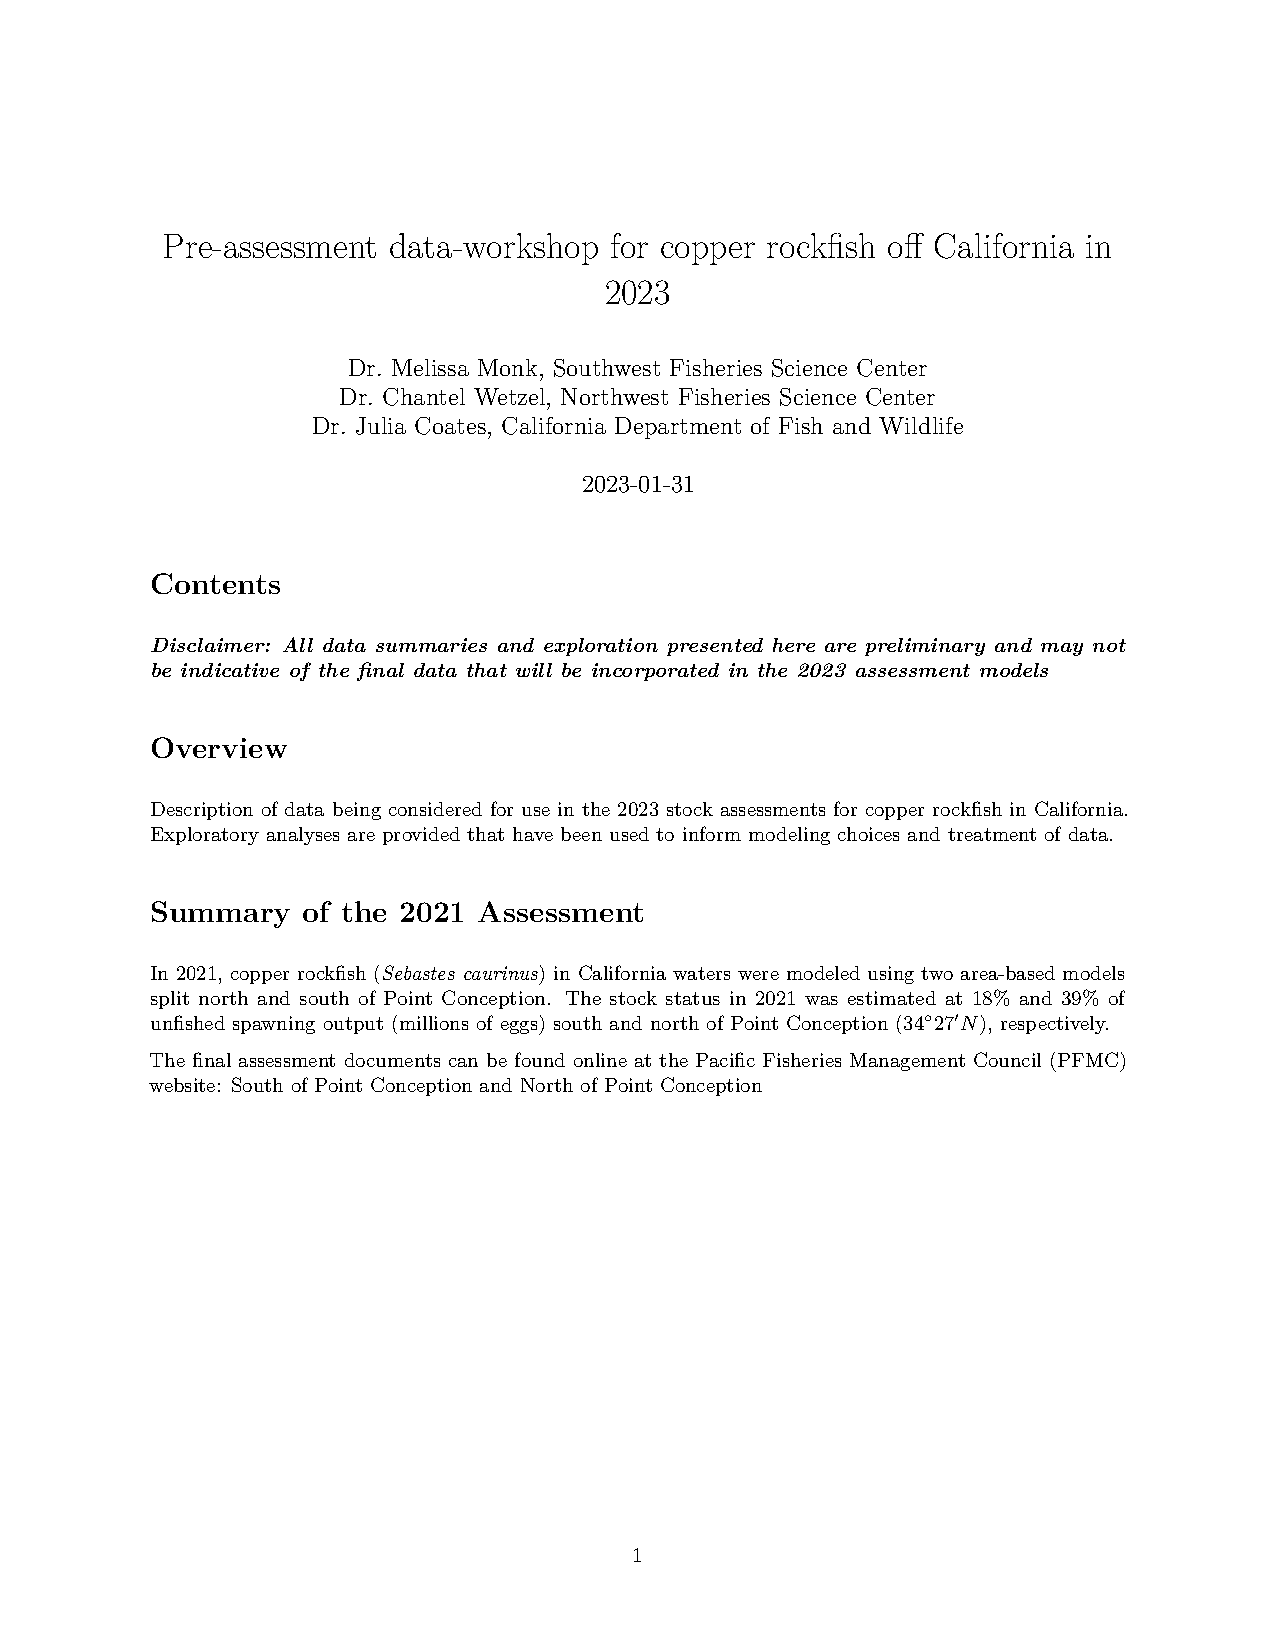
\includegraphics[width=1\textwidth,height=1\textheight]{S:/copper_rockfish_2023/data/rec_indices/crfs_pr_dockside/north/rm_last2yrs_area_weighted/index.png}
\caption{Index for the dockside PR survey.\label{fig:pr-index}}
\end{figure}

\newpage

\begin{figure}
\centering
\includegraphics[width=1\textwidth,height=1\textheight]{S:/copper_rockfish_2023/data/rec_indices/crfs_pr_dockside/north/rm_last2yrs_area_weighted/qq.png}
\caption{QQ plot for the dockside PR survey.\label{fig:pr-qq}}
\end{figure}

\newpage

\clearpage

\hypertarget{figures}{%
\section{Figures}\label{figures}}

\hypertarget{data}{%
\subsection{Data}\label{data}}

\begin{figure}
\centering
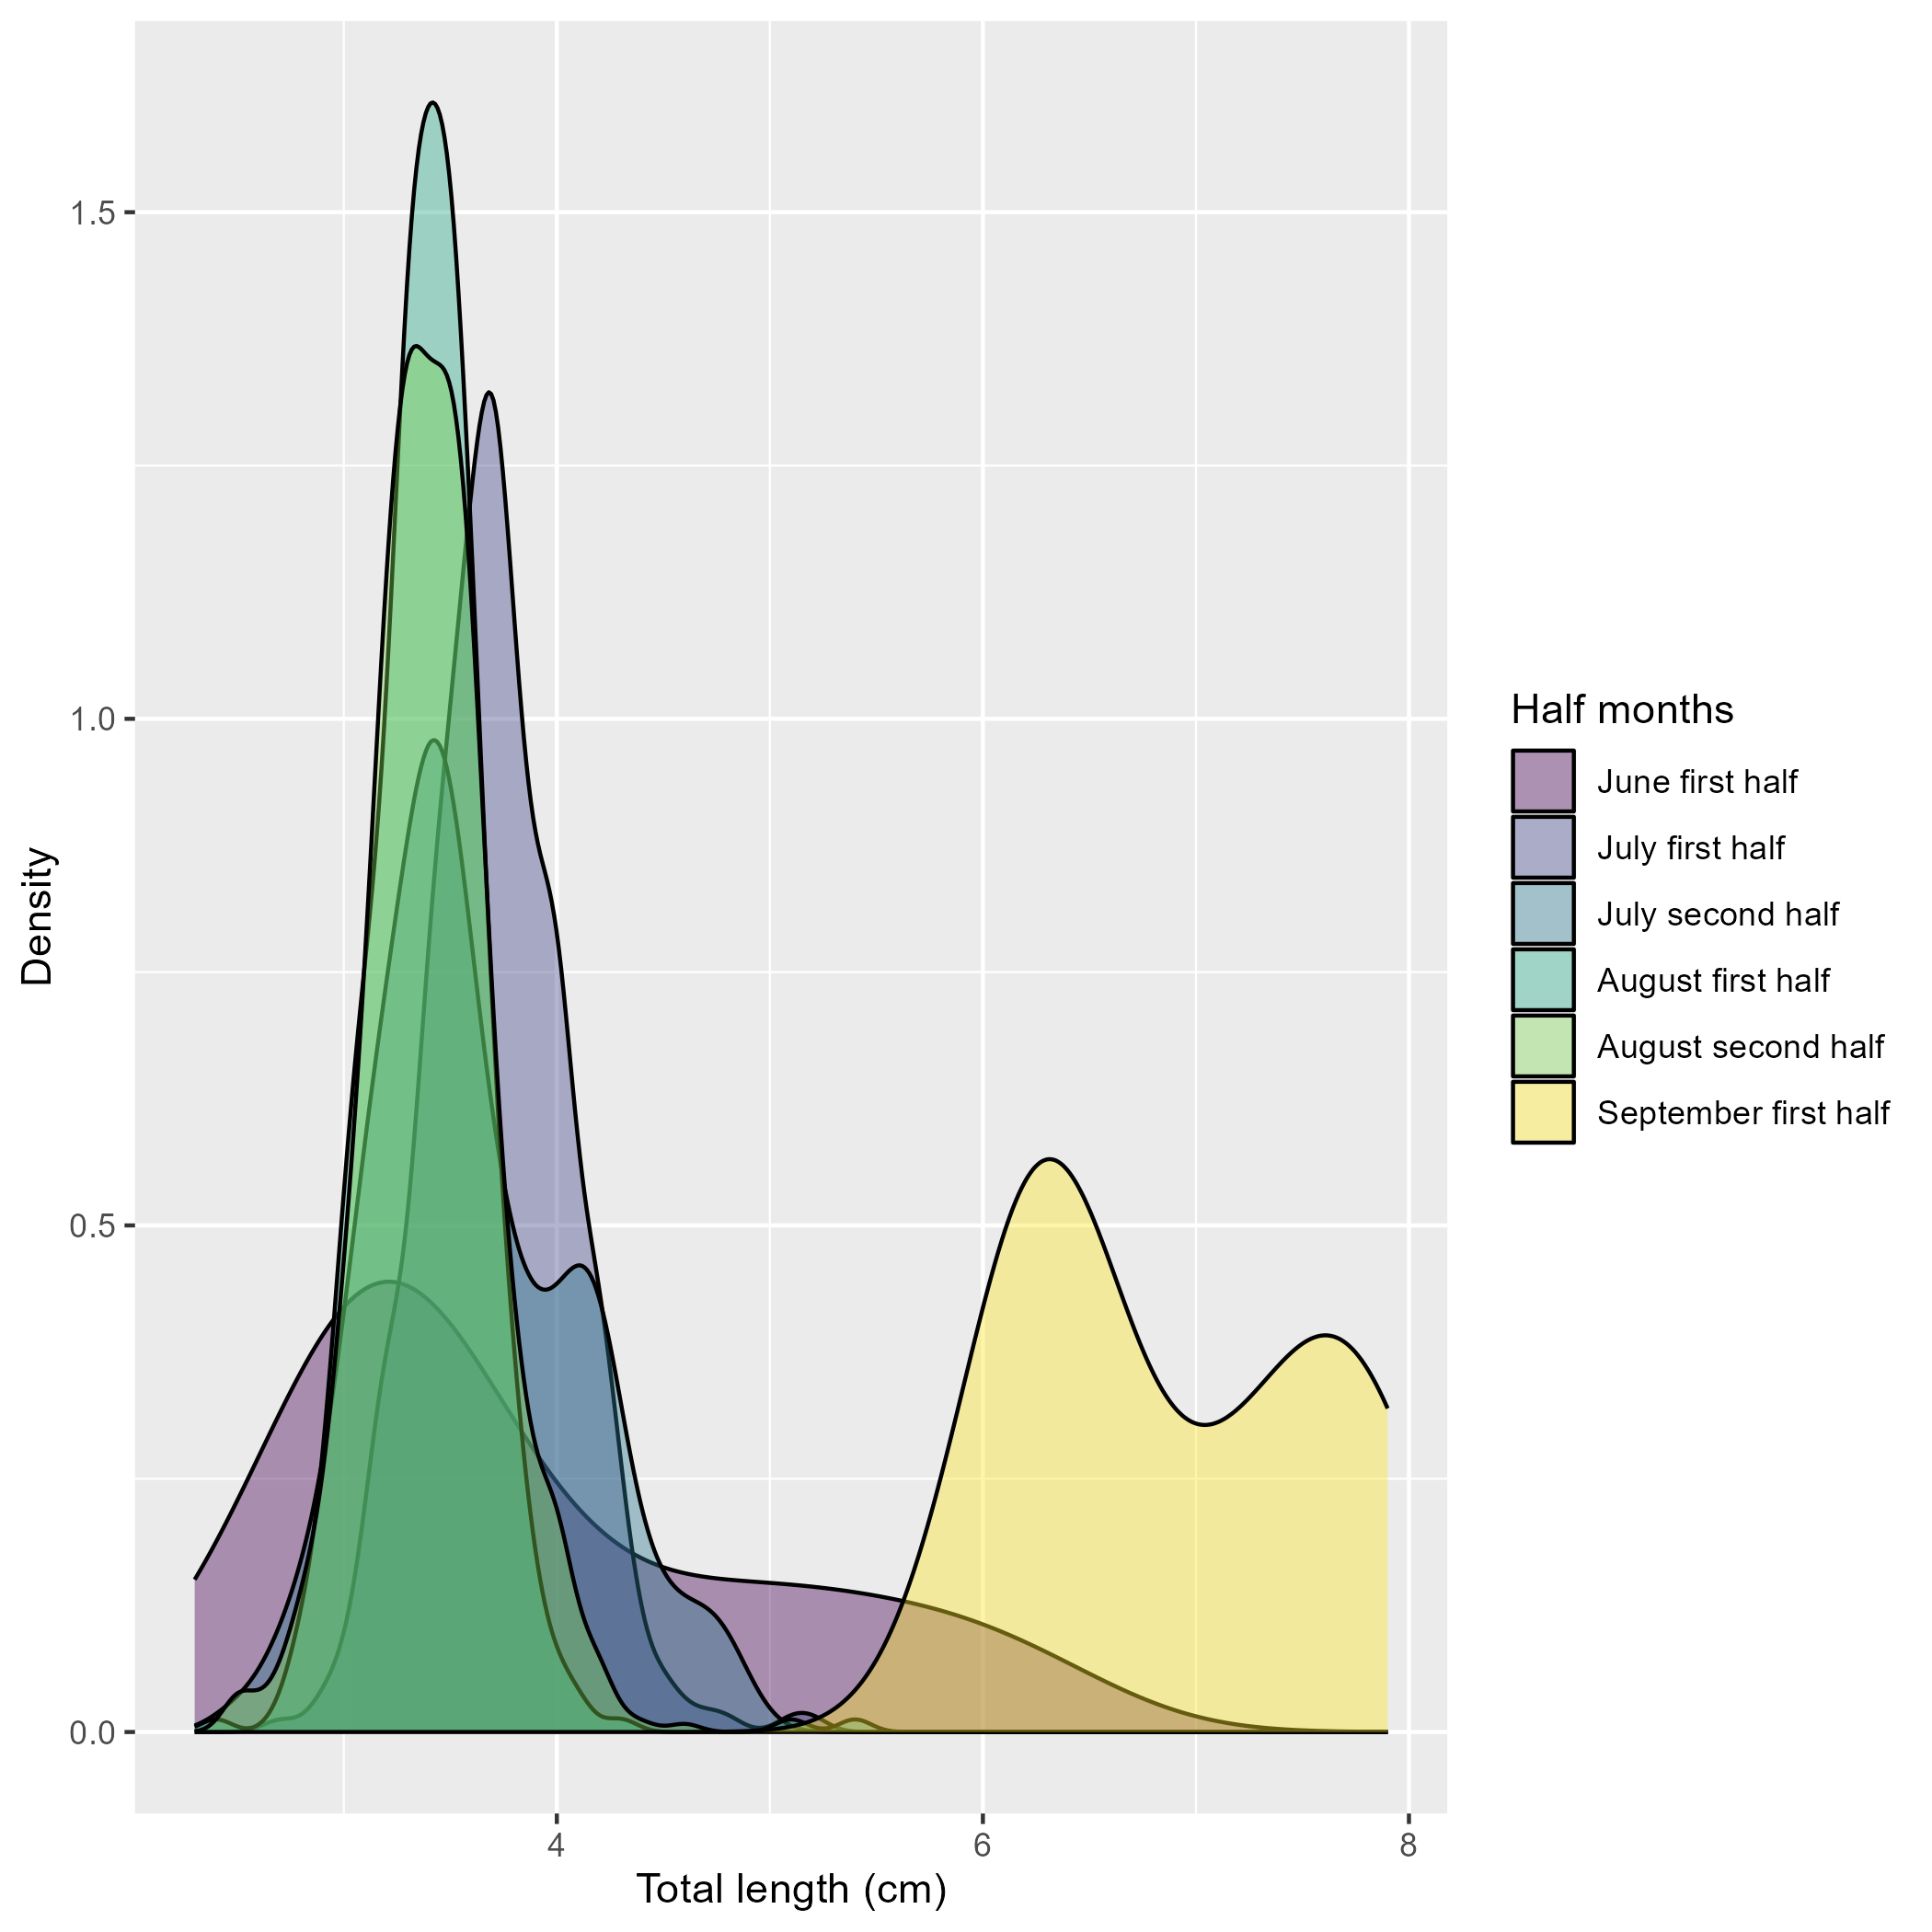
\includegraphics[width=1\textwidth,height=1\textheight]{C:/Users/melissa.monk/Documents/GitHub/copper_rockfish_2023/documents/shared_figures/copper_length_by_half_month.png}
\caption{Distribution of YOY copper rockfish lengths from fish genetically identified from D. Baetscher.\label{fig:copper-smurf-length}}
\end{figure}

\pagebreak

\begin{figure}
\centering
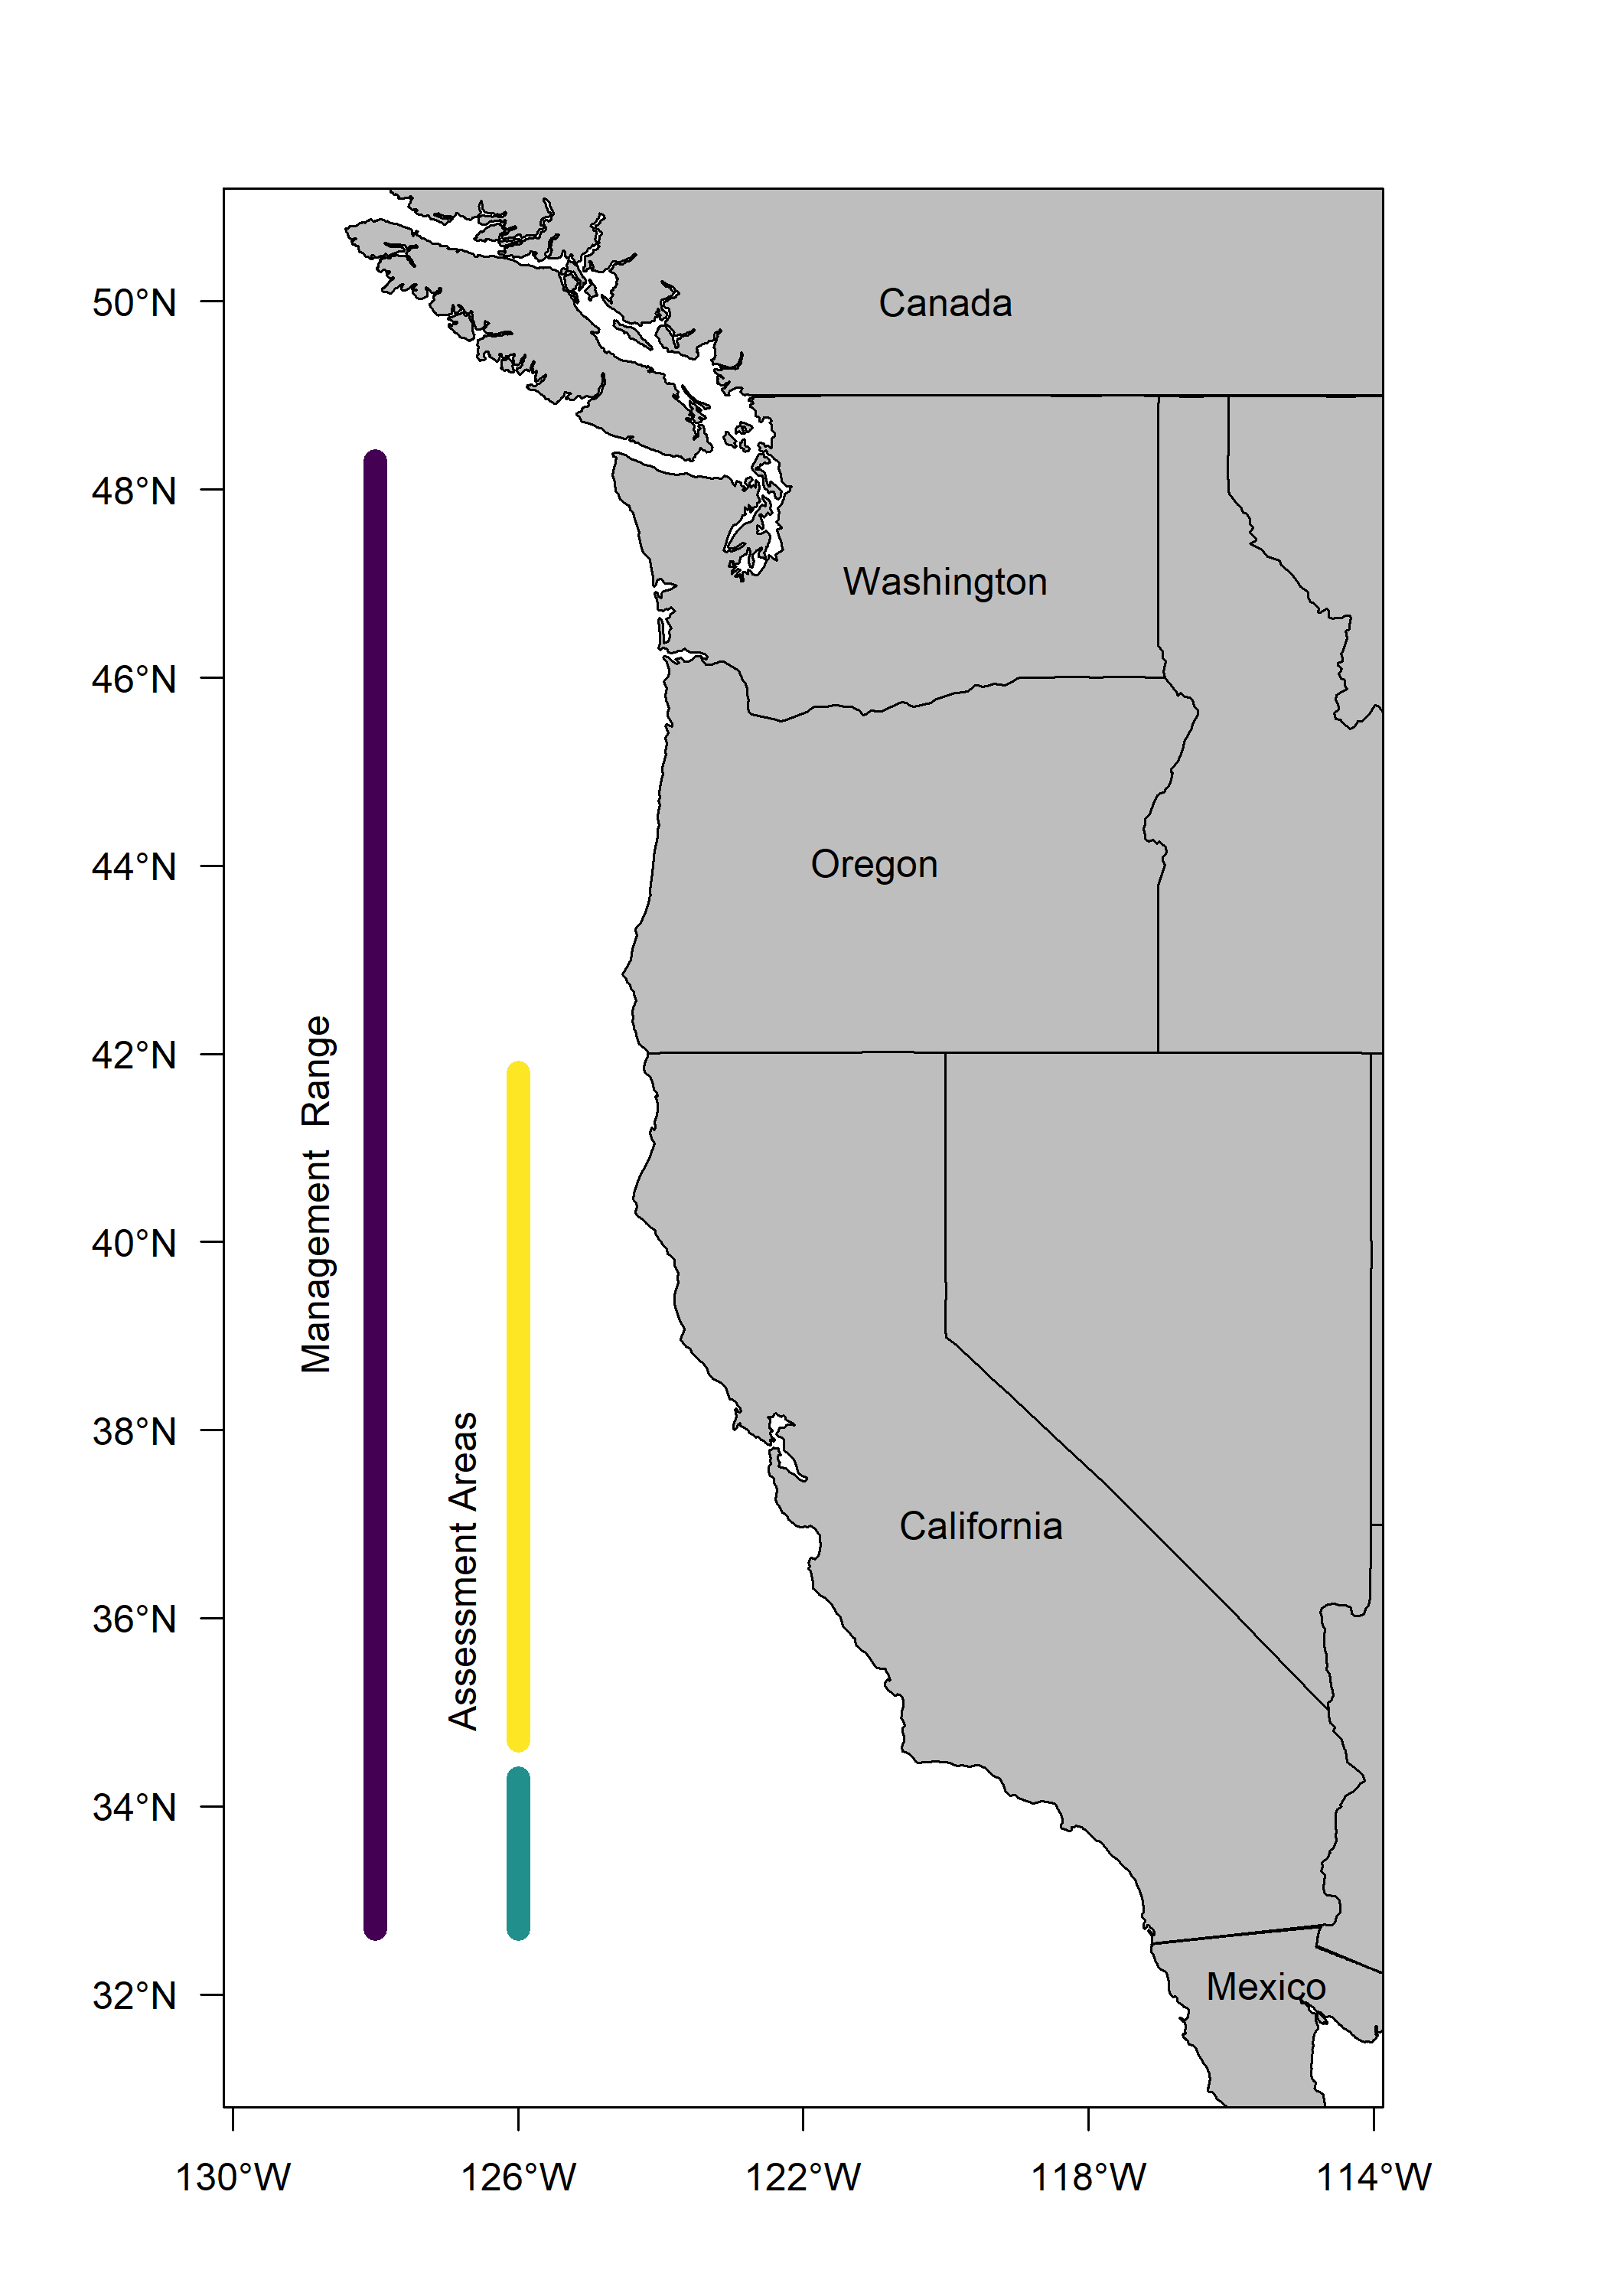
\includegraphics[width=1\textwidth,height=1\textheight]{C:/Users/melissa.monk/Documents/GitHub/copper_rockfish_2023/documents/shared_figures/map.png}
\caption{Map of management area and the 2023 assessments areas for copper rockfish.\label{fig:ca-map}}
\end{figure}

\pagebreak

\begin{figure}
\centering
\includegraphics[width=1\textwidth,height=1\textheight]{S:/copper_rockfish_2023/models/nca/9.8_selex_fix_forecast/plots/catch2 landings stacked.png}
\caption{Landings by fleet used in the base model where catches in metric tons by fleet are stacked.\label{fig:catch}}
\end{figure}

\pagebreak

\begin{figure}
\centering
\includegraphics[width=1\textwidth,height=1\textheight]{S:/copper_rockfish_2023/models/nca/9.8_selex_fix_forecast/plots/data_plot.png}
\caption{Summary of data sources used in the base model.\label{fig:data-plot}}
\end{figure}

\pagebreak

\begin{figure}
\centering
\includegraphics[width=1\textwidth,height=1\textheight]{S:/copper_rockfish_2023/models/nca/9.8_selex_fix_forecast/plots/comp_lendat_bubflt1mkt0.png}
\caption{Length composition data from the commercial dead fleet.\label{fig:com-dead-len-data}}
\end{figure}

\pagebreak

\begin{figure}
\centering
\includegraphics[width=1\textwidth,height=1\textheight]{S:/copper_rockfish_2023/models/nca/9.8_selex_fix_forecast/plots/comp_lendat_data_weighting_TA1.8_Commercial_Dead.png}
\caption{Mean length for commercial dead fleet with 95 percent confidence intervals.\label{fig:mean-com-dead-len-data}}
\end{figure}

\pagebreak

\begin{figure}
\centering
\includegraphics[width=1\textwidth,height=1\textheight]{S:/copper_rockfish_2023/models/nca/9.8_selex_fix_forecast/plots/comp_condAALdat_bubflt1mkt0.png}
\caption{Conditional age-at-length composition data from the commercial dead fleet.\label{fig:com-dead-age-data}}
\end{figure}

\pagebreak

\begin{figure}
\centering
\includegraphics[width=1\textwidth,height=1\textheight]{S:/copper_rockfish_2023/models/nca/9.8_selex_fix_forecast/plots/comp_lendat_bubflt2mkt0.png}
\caption{Length composition data from the commercial live fleet.\label{fig:com-live-len-data}}
\end{figure}

\pagebreak

\begin{figure}
\centering
\includegraphics[width=1\textwidth,height=1\textheight]{S:/copper_rockfish_2023/models/nca/9.8_selex_fix_forecast/plots/comp_lendat_data_weighting_TA1.8_Commercial_Live.png}
\caption{Mean length for commercial live fleet with 95 percent confidence intervals.\label{fig:mean-com-live-len-data}}
\end{figure}

\pagebreak

\begin{figure}
\centering
\includegraphics[width=1\textwidth,height=1\textheight]{S:/copper_rockfish_2023/data/rec_indices/mrfss_cpfv_dockside/north/forSS/Index.png}
\caption{Estimated annual index of abundances for the CPFV fleet based on MRFSS survey data.\label{fig:mrfss-index-main}}
\end{figure}

\pagebreak

\begin{figure}
\centering
\includegraphics[width=1\textwidth,height=1\textheight]{S:/copper_rockfish_2023/data/rec_indices/debwv_cpfv_onboard/deltalogn/Index.png}
\caption{Estimated annual index of abundances for the CPFV fleet based on the Deb Wilson-Vandenberg survey data.\label{fig:dwv-index-main}}
\end{figure}

\pagebreak

\begin{figure}
\centering
\includegraphics[width=1\textwidth,height=1\textheight]{S:/copper_rockfish_2023/data/rec_indices/crfs_cpfv_onboard/north/area_weighted/Index.png}
\caption{Estimated annual index of abundances for the CPFV fleet based on CRFS survey data.\label{fig:crfs-index-main}}
\end{figure}

\pagebreak

\begin{figure}
\centering
\includegraphics[width=1\textwidth,height=1\textheight]{S:/copper_rockfish_2023/data/rec_indices/crfs_pr_dockside/north/rm_last2yrs_area_weighted/Index.png}
\caption{Estimated annual index of abundances for the CPFV fleet based on CRFS survey data.\label{fig:crfs-pr-index-main}}
\end{figure}

\pagebreak

\begin{figure}
\centering
\includegraphics[width=1\textwidth,height=1\textheight]{S:/copper_rockfish_2023/models/nca/9.8_selex_fix_forecast/plots/comp_lendat_bubflt3mkt0_page2.png}
\caption{Length composition data from the recreational CPFV fleet.\label{fig:rec-cpfv-len-data}}
\end{figure}

\pagebreak

\begin{figure}
\centering
\includegraphics[width=1\textwidth,height=1\textheight]{S:/copper_rockfish_2023/models/nca/9.8_selex_fix_forecast/plots/comp_lendat_data_weighting_TA1.8_Rec_CPFV.png}
\caption{Mean length for recreational CPFV fleet with 95 percent confidence intervals.\label{fig:mean-rec-cpfv-len-data}}
\end{figure}

\pagebreak

\begin{figure}
\centering
\includegraphics[width=1\textwidth,height=1\textheight]{S:/copper_rockfish_2023/models/nca/9.8_selex_fix_forecast/plots/comp_condAALdat_bubflt3mkt0.png}
\caption{Conditional age-at-length composition data from the recreational CPFV fleet.\label{fig:rec-cpfv-caal-data}}
\end{figure}

\pagebreak

\begin{figure}
\centering
\includegraphics[width=1\textwidth,height=1\textheight]{S:/copper_rockfish_2023/models/nca/9.8_selex_fix_forecast/plots/comp_agedat_data_weighting_TA1.8_Rec_CPFV.png}
\caption{Mean age for recreational CPFV fleet with 95 percent confidence intervals.\label{fig:mean-rec-cpfv-age-data}}
\end{figure}

\pagebreak

\begin{figure}
\centering
\includegraphics[width=1\textwidth,height=1\textheight]{S:/copper_rockfish_2023/data/ages/plots/coop_crfs_length_comparison.png}
\caption{Comparison of all length collected by the CRFS sampling program for the CPFV fleet to the lengths from the fish with ages from the cooperative sampling program. The length distributions in the area north of Point Conception are in general agreement while the distribution of lengths collected by this program does not align with the length samples from CRFS.\label{fig:coop-len-comparison}}
\end{figure}

\pagebreak

\begin{figure}
\centering
\includegraphics[width=1\textwidth,height=1\textheight]{S:/copper_rockfish_2023/models/nca/9.8_selex_fix_forecast/plots/comp_condAALdat_bubflt4mkt0.png}
\caption{Conditional age-at-length data for recreational PR collected in 2022.\label{fig:rec-pr-caal-data}}
\end{figure}

\pagebreak

\begin{figure}
\centering
\includegraphics[width=1\textwidth,height=1\textheight]{S:/copper_rockfish_2023/models/nca/9.8_selex_fix_forecast/plots/comp_lendat_flt4mkt0_page2.png}
\caption{Length composition data from the recreational PR fleet.\label{fig:rec-pr-len-data}}
\end{figure}

\pagebreak

\begin{figure}
\centering
\includegraphics[width=1\textwidth,height=1\textheight]{S:/copper_rockfish_2023/models/nca/9.8_selex_fix_forecast/plots/comp_lendat_data_weighting_TA1.8_Rec_PR.png}
\caption{Mean length for recreational PR fleet with 95 percent confidence intervals.\label{fig:mean-rec-pr-len-data}}
\end{figure}

\pagebreak

\begin{figure}
\centering
\includegraphics[width=1\textwidth,height=1\textheight]{S:/copper_rockfish_2023/data/survey_indices/plots/north_survey_locations_designation.png}
\caption{Sample locations by each of the fishery-independent data sources used in the base model with indices of abundance, lengths, and ages if collected.\label{fig:survey-locations}}
\end{figure}

\pagebreak

\begin{figure}
\centering
\includegraphics[width=1\textwidth,height=1\textheight]{S:/copper_rockfish_2023/data/survey_indices/plots/north_survey_locations.png}
\caption{Sample locations by area, areas open to fishing (reference) and MPAS, for each of the fishery-independent data sources used in the base model with indices of abundance, lengths, and ages if collected.\label{fig:ref-mpa}}
\end{figure}

\pagebreak

\begin{figure}
\centering
\includegraphics[width=1\textwidth,height=1\textheight]{S:/copper_rockfish_2023/data/survey_indices/ccfrp/north/area_weighted/Index.png}
\caption{Estimated index of abundance from the CCFRP survey.\label{fig:ccfrp-index-main}}
\end{figure}

\pagebreak

\begin{figure}
\centering
\includegraphics[width=1\textwidth,height=1\textheight]{S:/copper_rockfish_2023/models/nca/9.8_selex_fix_forecast/plots/comp_lendat_bubflt5mkt0.png}
\caption{Length composition data from the CCFRP survey.\label{fig:ccfrp-len-data}}
\end{figure}

\pagebreak

\begin{figure}
\centering
\includegraphics[width=1\textwidth,height=1\textheight]{S:/copper_rockfish_2023/models/nca/9.8_selex_fix_forecast/plots/comp_lendat_data_weighting_TA1.8_CCFRP.png}
\caption{Mean length for the CCFRP survey with 95 percent confidence intervals.\label{fig:ccfrp-mean-len-data}}
\end{figure}

\pagebreak

\begin{figure}
\centering
\includegraphics[width=1\textwidth,height=1\textheight]{S:/copper_rockfish_2023/models/nca/9.8_selex_fix_forecast/plots/comp_condAALdat_bubflt5mkt0.png}
\caption{Conditional age-at-length data from the CCFRP survey.\label{fig:ccfrp-age-data}}
\end{figure}

\pagebreak

\begin{figure}
\centering
\includegraphics[width=1\textwidth,height=1\textheight]{S:/copper_rockfish_2023/data/survey_indices/rov/plots/rov_transect_collapsed_copper_north_protection_count.png}
\caption{The location and size of observations across all years and transects.\label{fig:rov-obs-loc}}
\end{figure}

\pagebreak

\begin{figure}
\centering
\includegraphics[width=1\textwidth,height=1\textheight]{S:/copper_rockfish_2023/data/survey_indices/rov/plots/north_raw_cpue_by_mpa_group.png}
\caption{The trend of the calculated CPUE by each MPA and Reference group.\label{fig:rov-raw-cpue}}
\end{figure}

\pagebreak

\begin{figure}
\centering
\includegraphics[width=1\textwidth,height=1\textheight]{S:/copper_rockfish_2023/data/survey_indices/rov/glm_negbin_north_designation_depth/Index.png}
\caption{The estimated weighted relative index of abundance.\label{fig:rov-index-main}}
\end{figure}

\pagebreak

\begin{figure}
\centering
\includegraphics[width=1\textwidth,height=1\textheight]{S:/copper_rockfish_2023/data/survey_indices/rov/plots/rov_length_by_area_designation.png}
\caption{The distribution of lengths across all years for MPA and Reference area north and south of Point Conception.\label{fig:rov-len}}
\end{figure}

\pagebreak

\begin{figure}
\centering
\includegraphics[width=1\textwidth,height=1\textheight]{S:/copper_rockfish_2023/models/nca/9.8_selex_fix_forecast/plots/comp_lendat_flt6mkt0.png}
\caption{Length composition data from the CDFW ROV survey.\label{fig:rov-len-data}}
\end{figure}

\pagebreak

\begin{figure}
\centering
\includegraphics[width=1\textwidth,height=1\textheight]{S:/copper_rockfish_2023/models/nca/9.8_selex_fix_forecast/plots/comp_lendat_data_weighting_TA1.8_CDFW_ROV.png}
\caption{Mean length for CDWF ROV survey with 95 percent confidence intervals.\label{fig:mean-rov-len-data}}
\end{figure}

\pagebreak

\begin{figure}
\centering
\includegraphics[width=1\textwidth,height=1\textheight]{S:/copper_rockfish_2023/data/ages/plots/south_growth_length_comparison.png}
\caption{Length distribution of fish by collection source that were used as conditional age-at-length data in the growth fleet.\label{fig:growth-len-dist}}
\end{figure}

\pagebreak

\begin{figure}
\centering
\includegraphics[width=1\textwidth,height=1\textheight]{S:/copper_rockfish_2023/data/ages/plots/south_growth_age_comparison.png}
\caption{Age distribution of fish by collection source that were used as conditional age-at-length data in the growth fleet.\label{fig:growth-age-dist}}
\end{figure}

\pagebreak

\begin{figure}
\centering
\includegraphics[width=1\textwidth,height=1\textheight]{S:/copper_rockfish_2023/data/wcgbt/north/plots/cpue_map.png}
\caption{Location and catch-per-unit-effort by location caught north of Point Conception by the NWFSC WCGBT survey.\label{fig:wcgbt-cpue}}
\end{figure}

\pagebreak

\begin{figure}
\centering
\includegraphics[width=1\textwidth,height=1\textheight]{S:/copper_rockfish_2023/data/wcgbt/north/plots/presence-absence_proportion_by_depth.png}
\caption{Number of positive tows across all years by depth in meters.\label{fig:wcgbt-depth}}
\end{figure}

\pagebreak

\begin{figure}
\centering
\includegraphics[width=1\textwidth,height=1\textheight]{S:/copper_rockfish_2023/data/wcgbt/plots/wcgbt_north_age_at_length_by_area.png}
\caption{Age and length by sex for copper rockfish caught north of Point Conception by the NWFSC WCGBT survey.\label{fig:wcgbt-len-age}}
\end{figure}

\pagebreak

\hypertarget{biology}{%
\subsection{Biology}\label{biology}}

\begin{figure}
\centering
\includegraphics[width=1\textwidth,height=1\textheight]{S:/copper_rockfish_2023/models/nca/9.8_selex_fix_forecast/plots/bio6_maturity.png}
\caption{Maturity as a function of length.\label{fig:maturity}}
\end{figure}

\pagebreak

\begin{figure}
\centering
\includegraphics[width=1\textwidth,height=1\textheight]{S:/copper_rockfish_2023/models/nca/9.8_selex_fix_forecast/plots/bio9_fecundity_len.png}
\caption{Fecundity as a function of length.\label{fig:fecundity}}
\end{figure}

\pagebreak

\begin{figure}
\centering
\includegraphics[width=1\textwidth,height=1\textheight]{S:/copper_rockfish_2023/data/wcgbt/plots/length_fraction_female.png}
\caption{Fraction of each sex by length by the NWFSC WCGBT survey.\label{fig:frac-sex-len}}
\end{figure}

\pagebreak

\begin{figure}
\centering
\includegraphics[width=1\textwidth,height=1\textheight]{S:/copper_rockfish_2023/data/biology/plots/Length_Weight_All.png}
\caption{Estimated weight-at-length.\label{fig:est-len-wght}}
\end{figure}

\pagebreak

\begin{figure}
\centering
\includegraphics[width=1\textwidth,height=1\textheight]{S:/copper_rockfish_2023/data/ages/ageing_error/B0_S3/Reader_1_vs_Reader_2.png}
\caption{Distribution of double reads between age reader 1 and 2.\label{fig:age-error-dist}}
\end{figure}

\pagebreak

\begin{figure}
\centering
\includegraphics[width=1\textwidth,height=1\textheight]{S:/copper_rockfish_2023/models/nca/9.8_selex_fix_forecast/plots/numbers5_ageerrorSD.png}
\caption{Ageing imprecision standard deviation of observed age in years.\label{fig:age-error}}
\end{figure}

\pagebreak

\begin{figure}
\centering
\includegraphics[width=1\textwidth,height=1\textheight]{S:/copper_rockfish_2023/models/nca/9.8_selex_fix_forecast/plots/numbers10_ageerror_matrix_1.png}
\caption{Distribution of observed age at true age for ageing error type 1.\label{fig:age-error-matrix}}
\end{figure}

\pagebreak

\hypertarget{model-results}{%
\subsection{Model Results}\label{model-results}}

\hypertarget{model-bridging}{%
\subsubsection{Model Bridging}\label{model-bridging}}

\begin{figure}
\centering
\includegraphics[width=1\textwidth,height=1\textheight]{S:/copper_rockfish_2023/models/nca/_bridging/_plots/0_model_convert_compare2_spawnbio_uncertainty.png}
\caption{Model version bridge comparison of estimated spawning output.\label{fig:bridge-ssb}}
\end{figure}

\pagebreak

\begin{figure}
\centering
\includegraphics[width=1\textwidth,height=1\textheight]{S:/copper_rockfish_2023/models/nca/_bridging/_plots/0_model_convert_compare4_Bratio_uncertainty.png}
\caption{Model version bridge comparison of estimated fraction unfished.\label{fig:bridge-depl}}
\end{figure}

\pagebreak

\begin{figure}
\centering
\includegraphics[width=1\textwidth,height=1\textheight]{S:/copper_rockfish_2023/models/nca/_bridging/_plots/full_bridge_1_compare2_spawnbio_uncertainty.png}
\caption{Model structure and data bridging comparison of estimated spawning output.\label{fig:data-bridge-ssb-1}}
\end{figure}

\pagebreak

\begin{figure}
\centering
\includegraphics[width=1\textwidth,height=1\textheight]{S:/copper_rockfish_2023/models/nca/_bridging/_plots/full_bridge_1_compare4_Bratio_uncertainty.png}
\caption{Model structure and data bridging comparison of estimated fraction unfished.\label{fig:data-bridge-depl-1}}
\end{figure}

\pagebreak

\begin{figure}
\centering
\includegraphics[width=1\textwidth,height=1\textheight]{S:/copper_rockfish_2023/models/nca/_bridging/_plots/full_bridge_2_compare2_spawnbio_uncertainty.png}
\caption{Model structure and data bridging comparison of estimated spawning output.\label{fig:data-bridge-ssb-2}}
\end{figure}

\pagebreak

\begin{figure}
\centering
\includegraphics[width=1\textwidth,height=1\textheight]{S:/copper_rockfish_2023/models/nca/_bridging/_plots/full_bridge_2_compare4_Bratio_uncertainty.png}
\caption{Model structure and data bridging comparison of estimated fraction unfished.\label{fig:data-bridge-depl-2}}
\end{figure}

\pagebreak

\pagebreak

\hypertarget{biology-1}{%
\subsubsection{Biology}\label{biology-1}}

\begin{figure}
\centering
\includegraphics[width=1\textwidth,height=1\textheight]{S:/copper_rockfish_2023/models/nca/9.8_selex_fix_forecast/plots/bio1_sizeatage.png}
\caption{Model estimated length-at-age in the beginning of the year. Shaded area indicates 95 percent distribution of length-at-age around the estimated growth curve.\label{fig:mod-est-len-age}}
\end{figure}

\pagebreak

\hypertarget{selectivity}{%
\subsubsection{Selectivity}\label{selectivity}}

\begin{figure}
\centering
\includegraphics[width=1\textwidth,height=1\textheight]{S:/copper_rockfish_2023/models/nca/9.8_selex_fix_forecast/plots/north_selectivity.png}
\caption{Estimated selectivity for each fleet and survey in the base model.\label{fig:est-selex}}
\end{figure}

\pagebreak

\hypertarget{recruitment}{%
\subsubsection{Recruitment}\label{recruitment}}

\begin{figure}
\centering
\includegraphics[width=1\textwidth,height=1\textheight]{S:/copper_rockfish_2023/models/nca/9.8_selex_fix_forecast/plots/ts11_Age-0_recruits_(1000s)_with_95_asymptotic_intervals.png}
\caption{Estimated time series of age-0 recruits (1000s).\label{fig:recruits}}
\end{figure}

\pagebreak

\begin{figure}
\centering
\includegraphics[width=1\textwidth,height=1\textheight]{S:/copper_rockfish_2023/models/nca/9.8_selex_fix_forecast/plots/recdevs2_withbars.png}
\caption{Estimated time series of recruitment deviations.\label{fig:rec-devs}}
\end{figure}

\pagebreak

\begin{figure}
\centering
\includegraphics[width=1\textwidth,height=1\textheight]{S:/copper_rockfish_2023/models/nca/9.8_selex_fix_forecast/plots/recruit_fit_bias_adjust.png}
\caption{Points are transformed variances. Red line shows current settings for bias adjustment specified in control file. Blue line shows least squares estimate of alternative bias adjustment relationship for recruitment deviations (which may or may not be an improvement).\label{fig:bias-adjust}}
\end{figure}

\newpage

\begin{figure}
\centering
\includegraphics[width=1\textwidth,height=1\textheight]{S:/copper_rockfish_2023/models/nca/9.8_selex_fix_forecast/plots/SR_curve.png}
\caption{Stock-recruit curve. Point colors indicate year, with warmer colors indicating earlier years and cooler colors in showing later years.\label{fig:bh-curve}}
\end{figure}

\pagebreak

\hypertarget{fits-to-data}{%
\subsubsection{Fits to Data}\label{fits-to-data}}

\begin{figure}
\centering
\includegraphics[width=1\textwidth,height=1\textheight]{S:/copper_rockfish_2023/models/nca/9.8_selex_fix_forecast/plots/comp_lenfit__aggregated_across_time.png}
\caption{Length composition aggregated across years by fleet with the model estimated fit to the data by sex (green unsexed, red female, and blue male).\label{fig:len-agg-fit}}
\end{figure}

\pagebreak

\begin{figure}
\centering
\includegraphics[width=1\textwidth,height=1\textheight]{S:/copper_rockfish_2023/models/nca/9.8_selex_fix_forecast/plots/comp_lenfit_residsflt1mkt0.png}
\caption{Pearson residuals for commercial fleet. Closed bubble are positive residuals (observed \textgreater{} expected) and open bubbles are negative residuals (observed \textless{} expected).\label{fig:com-dead-pearson}}
\end{figure}

\pagebreak

\begin{figure}
\centering
\includegraphics[width=1\textwidth,height=1\textheight]{S:/copper_rockfish_2023/models/nca/9.8_selex_fix_forecast/plots/comp_lenfit_data_weighting_TA1.8_Commercial_dead.png}
\caption{Mean length for commercial dead lengths with 95 percent confidence intervals based on current samples sizes.\label{fig:com-dead-mean-len-fit}}
\end{figure}

\pagebreak

\pagebreak

\begin{figure}
\centering
\includegraphics[width=1\textwidth,height=1\textheight]{S:/copper_rockfish_2023/models/nca/9.8_selex_fix_forecast/plots/comp_lenfit_residsflt2mkt0.png}
\caption{Pearson residuals for commercial live fleet. Closed bubble are positive residuals (observed \textgreater{} expected) and open bubbles are negative residuals (observed \textless{} expected).\label{fig:com-live-pearson}}
\end{figure}

\pagebreak

\begin{figure}
\centering
\includegraphics[width=1\textwidth,height=1\textheight]{S:/copper_rockfish_2023/models/nca/9.8_selex_fix_forecast/plots/comp_lenfit_data_weighting_TA1.8_Commercial_live.png}
\caption{Mean length for commercial live fish lengths with 95 percent confidence intervals based on current samples sizes.\label{fig:com-live-mean-len-fit}}
\end{figure}

\pagebreak

\begin{figure}
\centering
\includegraphics[width=1\textwidth,height=1\textheight]{S:/copper_rockfish_2023/models/nca/9.8_selex_fix_forecast/plots/comp_lenfit_residsflt3mkt0_page2.png}
\caption{Pearson residuals for recreational CPFV fleet. Closed bubble are positive residuals (observed \textgreater{} expected) and open bubbles are negative residuals (observed \textless{} expected).\label{fig:rec-cpfv-pearson}}
\end{figure}

\pagebreak

\begin{figure}
\centering
\includegraphics[width=1\textwidth,height=1\textheight]{S:/copper_rockfish_2023/models/nca/9.8_selex_fix_forecast/plots/comp_lenfit_data_weighting_TA1.8_Rec_CPFV.png}
\caption{Mean length for recreational CPFV lengths with 95 percent confidence intervals based on current samples sizes.\label{fig:rec-cpfv-mean-len-fit}}
\end{figure}

\pagebreak

\begin{figure}
\centering
\includegraphics[width=1\textwidth,height=1\textheight]{S:/copper_rockfish_2023/models/nca/9.8_selex_fix_forecast/plots/comp_agefit_residsflt3mkt0.png}
\caption{Pearson residuals for recreational CPFV age data. Closed bubble are positive residuals (observed \textgreater{} expected) and open bubbles are negative residuals (observed \textless{} expected).\label{fig:rec-cpfv-age-pearson}}
\end{figure}

\pagebreak

\begin{figure}
\centering
\includegraphics[width=1\textwidth,height=1\textheight]{S:/copper_rockfish_2023/models/nca/9.8_selex_fix_forecast/plots/comp_lenfit_residsflt4mkt0_page2.png}
\caption{Pearson residuals for recreational private/rental fleet. Closed bubble are positive residuals (observed \textgreater{} expected) and open bubbles are negative residuals (observed \textless{} expected).\label{fig:rec-pr-pearson}}
\end{figure}

\pagebreak

\begin{figure}
\centering
\includegraphics[width=1\textwidth,height=1\textheight]{S:/copper_rockfish_2023/models/nca/9.8_selex_fix_forecast/plots/comp_lenfit_data_weighting_TA1.8_Rec_PR.png}
\caption{Mean length for recreational private/rental lengths with 95 percent confidence intervals based on current samples sizes.\label{fig:rec-pr-mean-len-fit}}
\end{figure}

\pagebreak

\begin{figure}
\centering
\includegraphics[width=1\textwidth,height=1\textheight]{S:/copper_rockfish_2023/models/nca/9.8_selex_fix_forecast/plots/comp_condAALfit_residsflt4mkt0.png}
\caption{Pearson residuals for the recreational private/rental conditional age-at-ength data. Closed bubble are positive residuals (observed \textgreater{} expected) and open bubbles are negative residuals (observed \textless{} expected).\label{fig:rec-pr-age-pearson}}
\end{figure}

\begin{figure}
\centering
\includegraphics[width=1\textwidth,height=1\textheight]{S:/copper_rockfish_2023/models/nca/9.8_selex_fix_forecast/plots/comp_lenfit_residsflt5mkt0.png}
\caption{Pearson residuals for CCFRP Hook and Line survey length data. Closed bubble are positive residuals (observed \textgreater{} expected) and open bubbles are negative residuals (observed \textless{} expected).\label{fig:ccfrp-len-pearson}}
\end{figure}

\pagebreak

\begin{figure}
\centering
\includegraphics[width=1\textwidth,height=1\textheight]{S:/copper_rockfish_2023/models/nca/9.8_selex_fix_forecast/plots/comp_lenfit_data_weighting_TA1.8_CCFRP.png}
\caption{Mean length for CCFRP Hook and Line survey lengths with 95 percent confidence intervals based on current samples sizes.\label{fig:ccfrp-mean-len-fit}}
\end{figure}

\pagebreak

\begin{figure}
\centering
\includegraphics[width=1\textwidth,height=1\textheight]{S:/copper_rockfish_2023/models/nca/9.8_selex_fix_forecast/plots/comp_condAAlfit_residsflt5mkt0.png}
\caption{Pearson residuals for CCFRP Hook and Line survey conditional-age-at-length data. Closed bubble are positive residuals (observed \textgreater{} expected) and open bubbles are negative residuals (observed \textless{} expected).\label{fig:ccfrp-age-pearson}}
\end{figure}

\pagebreak

\begin{figure}
\centering
\includegraphics[width=1\textwidth,height=1\textheight]{S:/copper_rockfish_2023/models/nca/9.8_selex_fix_forecast/plots/comp_lenfit_residsflt6mkt0.png}
\caption{Pearson residuals for CDFW ROV survey length data. Closed bubble are positive residuals (observed \textgreater{} expected) and open bubbles are negative residuals (observed \textless{} expected).\label{fig:rov-pearson}}
\end{figure}

\pagebreak

\begin{figure}
\centering
\includegraphics[width=1\textwidth,height=1\textheight]{S:/copper_rockfish_2023/models/nca/9.8_selex_fix_forecast/plots/comp_lenfit_data_weighting_TA1.8_CDFW_ROV.png}
\caption{Mean length for CDFW ROV survey lengths with 95 percent confidence intervals based on current samples sizes.\label{fig:rov-mean-len-fit}}
\end{figure}

\pagebreak

\begin{figure}
\centering
\includegraphics[width=1\textwidth,height=1\textheight]{S:/copper_rockfish_2023/models/nca/9.8_selex_fix_forecast/plots/index5_logcpuefit_Rec_CPFV.png}
\caption{Fit to log index data on log scale for recreational (MRFSS) CPFV. Lines indicate 95\% uncertainty interval around index values based on the model assumption of lognormal error. Thicker lines (if present) indicate input uncertainty before addition of estimated additional uncertainty parameter.\label{fig:mrfss-cpfv-index-fit}}
\end{figure}

\pagebreak

\begin{figure}
\centering
\includegraphics[width=1\textwidth,height=1\textheight]{S:/copper_rockfish_2023/models/nca/9.8_selex_fix_forecast/plots/index5_logcpuefit_DWV_CPFV.png}
\caption{Fit to log index data on log scale for Deb Wilson-Vandenberg CPFV survey. Lines indicate 95\% uncertainty interval around index values based on the model assumption of lognormal error. Thicker lines (if present) indicate input uncertainty before addition of estimated additional uncertainty parameter.\label{fig:dwv-cpfv-index-fit}}
\end{figure}

\pagebreak

\begin{figure}
\centering
\includegraphics[width=1\textwidth,height=1\textheight]{S:/copper_rockfish_2023/models/nca/9.8_selex_fix_forecast/plots/index5_logcpuefit_CRFS_CPFV.png}
\caption{Fit to log index data on log scale for CRFS CPFV survey. Lines indicate 95\% uncertainty interval around index values based on the model assumption of lognormal error. Thicker lines (if present) indicate input uncertainty before addition of estimated additional uncertainty parameter.\label{fig:crfs-cpfv-index-fit}}
\end{figure}

\pagebreak

\begin{figure}
\centering
\includegraphics[width=1\textwidth,height=1\textheight]{S:/copper_rockfish_2023/models/nca/9.8_selex_fix_forecast/plots/index5_logcpuefit_Rec_PR.png}
\caption{Fit to log index data on log scale for recreational (CRFS) PR. Lines indicate 95\% uncertainty interval around index values based on the model assumption of lognormal error. Thicker lines (if present) indicate input uncertainty before addition of estimated additional uncertainty parameter.\label{fig:crfs-pr-index-fit}}
\end{figure}

\pagebreak

\begin{figure}
\centering
\includegraphics[width=1\textwidth,height=1\textheight]{S:/copper_rockfish_2023/models/nca/9.8_selex_fix_forecast/plots/index5_logcpuefit_CCFRP.png}
\caption{Fit to log index data on log scale for CCFRP survey. Lines indicate 95\% uncertainty interval around index values based on the model assumption of lognormal error. Thicker lines (if present) indicate input uncertainty before addition of estimated additional uncertainty parameter.\label{fig:ccfrp-index-fit}}
\end{figure}

\pagebreak

\begin{figure}
\centering
\includegraphics[width=1\textwidth,height=1\textheight]{S:/copper_rockfish_2023/models/nca/9.8_selex_fix_forecast/plots/index5_logcpuefit_CDFW_ROV.png}
\caption{Fit to log index data on log scale for CDFW ROV survey. Lines indicate 95\% uncertainty interval around index values based on the model assumption of lognormal error. Thicker lines (if present) indicate input uncertainty before addition of estimated additional uncertainty parameter.\label{fig:rov-index-fit}}
\end{figure}

\pagebreak

\begin{figure}
\centering
\includegraphics[width=1\textwidth,height=1\textheight]{S:/copper_rockfish_2023/models/nca/9.8_selex_fix_forecast/plots/index9_standcpueall.png}
\caption{Standardized indices overlaid. Each index is rescaled to have mean observation = 1.0.\label{fig:standardized-indices}}
\end{figure}

\pagebreak

\hypertarget{time-series}{%
\subsubsection{Time-series}\label{time-series}}

\begin{figure}
\centering
\includegraphics[width=1\textwidth,height=1\textheight]{S:/copper_rockfish_2023/models/nca/9.8_selex_fix_forecast/plots/ts7_Spawning_output_with_95_asymptotic_intervals_intervals.png}
\caption{Estimated time series of spawning biomass.\label{fig:ssb}}
\end{figure}

\pagebreak

\begin{figure}
\centering
\includegraphics[width=1\textwidth,height=1\textheight]{S:/copper_rockfish_2023/models/nca/9.8_selex_fix_forecast/plots/ts1_Total_biomass_(mt).png}
\caption{Estimated time series of total biomass.\label{fig:tot-bio}}
\end{figure}

\pagebreak

\begin{figure}
\centering
\includegraphics[width=1\textwidth,height=1\textheight]{S:/copper_rockfish_2023/models/nca/9.8_selex_fix_forecast/plots/ts9_Relative_spawning_output_intervals.png}
\caption{Estimated time series of fraction of unfished spawning biomass.\label{fig:depl}}
\end{figure}

\pagebreak

\begin{figure}
\centering
\includegraphics[width=1\textwidth,height=1\textheight]{C:/Users/melissa.monk/Documents/GitHub/copper_rockfish_2023/documents/shared_figures/spawning_output_combined.png}
\caption{Estimated combined time series of spawning output for copper rockfish in California waters.\label{fig:sb-all}}
\end{figure}

\clearpage

\begin{figure}
\centering
\includegraphics[width=1\textwidth,height=1\textheight]{C:/Users/melissa.monk/Documents/GitHub/copper_rockfish_2023/documents/shared_figures/depletion_combined.png}
\caption{Estimated combined time series of fraction of relative spawning output for copper rockfish in California waters.\label{fig:depl-all}}
\end{figure}

\clearpage

\hypertarget{sensitivity-analyses-and-retrospectives}{%
\subsubsection{Sensitivity Analyses and Retrospectives}\label{sensitivity-analyses-and-retrospectives}}

\begin{figure}
\centering
\includegraphics[width=1\textwidth,height=1\textheight]{S:/copper_rockfish_2023/models/nca/_sensitivities/_plots/Sensi_REplot_all_horizontal}
\caption{Comparison of the relative change in estimated management quantities as compared to the base model. The quantities compared are the estimate of unfished spawning biomass (SB0), spawning output in 2023 (SB2023), the relative spawnin output (SB2023/SB0), the yield based on a spawner per recruit harvest rate (YieldSPR=0.50), and the fishing mortality at that harvest rate (FSPR=0.50). The colored boxes indicate the 95 percent confidence interval around the point estimate of the quantity from the base model where each color corresponds with a specific quantity in the legend. A model with matching estimates as the base model would reflect a relative change of 0, a model with estimates less than the base model would have a negative relative change, and a model with estimates greater than the base model would have a positive relative change.\label{fig:sens-all}}
\end{figure}

\newpage

\begin{figure}
\centering
\includegraphics[width=1\textwidth,height=1\textheight]{S:/copper_rockfish_2023/models/nca/_sensitivities/_plots/9.8_selex_fix_forecast_final_1_compare2_spawnbio_uncertainty.png}
\caption{Change in estimated spawning output by sensitivity.\label{fig:sens-ssb-1}}
\end{figure}

\newpage

\begin{figure}
\centering
\includegraphics[width=1\textwidth,height=1\textheight]{S:/copper_rockfish_2023/models/nca/_sensitivities/_plots/9.8_selex_fix_forecast_final_1_compare4_Bratio_uncertainty.png}
\caption{Change in estimated fraction unfished by sensitivity.\label{fig:sens-depl-1}}
\end{figure}

\newpage

\begin{figure}
\centering
\includegraphics[width=1\textwidth,height=1\textheight]{S:/copper_rockfish_2023/models/nca/_sensitivities/_plots/9.8_selex_fix_forecast_final_2_compare2_spawnbio_uncertainty.png}
\caption{Change in estimated spawning output by sensitivity.\label{fig:sens-ssb-2}}
\end{figure}

\newpage

\begin{figure}
\centering
\includegraphics[width=1\textwidth,height=1\textheight]{S:/copper_rockfish_2023/models/nca/_sensitivities/_plots/9.8_selex_fix_forecast_final_2_compare4_Bratio_uncertainty.png}
\caption{Change in estimated fraction unfished by sensitivity.\label{fig:sens-depl-2}}
\end{figure}

\newpage

\begin{figure}
\centering
\includegraphics[width=1\textwidth,height=1\textheight]{S:/copper_rockfish_2023/models/nca/_sensitivities/_plots/9.8_selex_fix_forecast_final_3_compare2_spawnbio_uncertainty.png}
\caption{Change in estimated spawning output by sensitivity.\label{fig:sens-ssb-3}}
\end{figure}

\newpage

\begin{figure}
\centering
\includegraphics[width=1\textwidth,height=1\textheight]{S:/copper_rockfish_2023/models/nca/_sensitivities/_plots/9.8_selex_fix_forecast_final_3_compare4_Bratio_uncertainty.png}
\caption{Change in estimated fraction unfished by sensitivity.\label{fig:sens-depl-3}}
\end{figure}

\newpage

\begin{figure}
\centering
\includegraphics[width=1\textwidth,height=1\textheight]{S:/copper_rockfish_2023/models/nca/9.8_selex_fix_forecast_retro/compare2_spawnbio_uncertainty.png}
\caption{Change in the estimate of spawning output when the most recent 5 years of data area removed sequentially.\label{fig:retro-ssb}}
\end{figure}

\pagebreak

\begin{figure}
\centering
\includegraphics[width=1\textwidth,height=1\textheight]{S:/copper_rockfish_2023/models/nca/9.8_selex_fix_forecast_retro/compare4_Bratio_uncertainty.png}
\caption{Change in the estimate of fraction unfished when the most recent 5 years of data area removed sequentially.\label{fig:retro-depl}}
\end{figure}

\pagebreak

\hypertarget{likelihood-profiles}{%
\subsubsection{Likelihood Profiles}\label{likelihood-profiles}}

\begin{figure}
\centering
\includegraphics[width=1\textwidth,height=1\textheight]{S:/copper_rockfish_2023/models/nca/9.8_selex_fix_forecast_profile_SR_LN(R0)_prior_like_0/piner_panel_SR_LN(R0).png}
\caption{Change in the negative log-likelihood across a range of log(R\textsubscript{0}) values.\label{fig:r0-profile}}
\end{figure}

\pagebreak

\begin{figure}
\centering
\includegraphics[width=1\textwidth,height=1\textheight]{S:/copper_rockfish_2023/models/nca/9.8_selex_fix_forecast_profile_SR_LN(R0)_prior_like_0/SR_LN(R0)_trajectories_compare1_spawnbio.png}
\caption{Change in the estimate of spawning output across a range of log(R\textsubscript{0}) values.\label{fig:r0-ssb}}
\end{figure}

\pagebreak

\begin{figure}
\centering
\includegraphics[width=1\textwidth,height=1\textheight]{S:/copper_rockfish_2023/models/nca/9.8_selex_fix_forecast_profile_SR_LN(R0)_prior_like_0/SR_LN(R0)_trajectories_compare3_Bratio.png}
\caption{Change in the estimate of fraction unfished across a range of log(R\textsubscript{0}) values.\label{fig:r0-depl}}
\end{figure}

\pagebreak

\begin{figure}
\centering
\includegraphics[width=1\textwidth,height=1\textheight]{S:/copper_rockfish_2023/models/nca/9.8_selex_fix_forecast_profile_SR_BH_steep_prior_like_1/piner_panel_SR_BH_steep.png}
\caption{Change in the negative log-likelihood across a range of steepness values.\label{fig:h-profile}}
\end{figure}

\pagebreak

\begin{figure}
\centering
\includegraphics[width=1\textwidth,height=1\textheight]{S:/copper_rockfish_2023/models/nca/9.8_selex_fix_forecast_profile_SR_BH_steep_prior_like_1/SR_BH_steep_trajectories_compare1_spawnbio.png}
\caption{Change in the estimate of spawning output across a range of steepness values.\label{fig:h-ssb}}
\end{figure}

\pagebreak

\begin{figure}
\centering
\includegraphics[width=1\textwidth,height=1\textheight]{S:/copper_rockfish_2023/models/nca/9.8_selex_fix_forecast_profile_SR_BH_steep_prior_like_1/SR_BH_steep_trajectories_compare3_Bratio.png}
\caption{Change in the estimate of fraction unfished across a range of steepness values.\label{fig:h-depl}}
\end{figure}

\pagebreak

\begin{figure}
\centering
\includegraphics[width=1\textwidth,height=1\textheight]{S:/copper_rockfish_2023/models/nca/9.8_selex_fix_forecast_profile_NatM_uniform_Fem_GP_1_prior_like_1/piner_panel_NatM_uniform_Fem_GP_1.png}
\caption{Change in the negative log-likelihood across a range of female natural mortality values.\label{fig:m-profile}}
\end{figure}

\pagebreak

\begin{figure}
\centering
\includegraphics[width=1\textwidth,height=1\textheight]{S:/copper_rockfish_2023/models/nca/9.8_selex_fix_forecast_profile_NatM_uniform_Fem_GP_1_prior_like_1/NatM_uniform_Fem_GP_1_trajectories_compare1_spawnbio.png}
\caption{Change in the estimate of spawning output across a range of female natural mortality values.\label{fig:m-ssb}}
\end{figure}

\pagebreak

\begin{figure}
\centering
\includegraphics[width=1\textwidth,height=1\textheight]{S:/copper_rockfish_2023/models/nca/9.8_selex_fix_forecast_profile_NatM_uniform_Fem_GP_1_prior_like_1/NatM_uniform_Fem_GP_1_trajectories_compare3_Bratio.png}
\caption{Change in the estimate of fraction unfished across a range of female natural values.\label{fig:m-depl}}
\end{figure}

\begin{figure}
\centering
\includegraphics[width=1\textwidth,height=1\textheight]{C:/Users/melissa.monk/Documents/GitHub/copper_rockfish_2023/documents/shared_figures/north_assess_compare_compare2_spawnbio_uncertainty.png}
\caption{Comparison of the estimated spawning output for the base model to previous assessment in 2021.\label{fig:comp-assess-sb}}
\end{figure}

\newpage

\begin{figure}
\centering
\includegraphics[width=1\textwidth,height=1\textheight]{C:/Users/melissa.monk/Documents/GitHub/copper_rockfish_2023/documents/shared_figures/north_assess_compare_compare4_Bratio_uncertainty.png}
\caption{Comparison of the estimated fraction unfished for the base model to previous assessment in 2021.\label{fig:comp-assess-depl}}
\end{figure}

\newpage

\hypertarget{reference-points-and-forecasts}{%
\subsubsection{Reference Points and Forecasts}\label{reference-points-and-forecasts}}

\begin{figure}
\centering
\includegraphics[width=1\textwidth,height=1\textheight]{C:/Users/melissa.monk/Documents/GitHub/copper_rockfish_2023/documents/shared_figures/compare6_SPRratio_uncertainty.png}
\caption{Estimated 1 - relative spawning ratio (SPR) by year for both sub-area models south and north of Point Conception.\label{fig:1-spr}}
\end{figure}

\clearpage

\begin{figure}
\centering
\includegraphics[width=1\textwidth,height=1\textheight]{C:/Users/melissa.monk/Documents/GitHub/copper_rockfish_2023/documents/shared_figures/compare15_phase_plot.png}
\caption{Phase plot of the relative biomass (also referred to as fraction unfished) versus the SPR ratio where each point represents the biomass ratio at the start of the year and the relative fishing intensity in that same year. Lines through the final point show the 95 percent intervals based on the asymptotic uncertainty for each dimension. The shaded ellipse is a 95 percent region which accounts for the estimated correlations between the biomass ratio and SPR ratio.\label{fig:phase}}
\end{figure}

\pagebreak

\begin{figure}
\centering
\includegraphics[width=1\textwidth,height=1\textheight]{S:/copper_rockfish_2023/models/sca/14.0_base_forecast/plots/yield2_yield_curve_with_refpoints.png}
\caption{Equilibrium yield curve for the base case model south of Point Conception. Values are based on the 2022
fishery selectivities and with steepness fixed at 0.72.\label{fig:yield-south}}
\end{figure}

\pagebreak

\begin{figure}
\centering
\includegraphics[width=1\textwidth,height=1\textheight]{S:/copper_rockfish_2023/models/nca/9.8_selex_fix_forecast/plots/yield2_yield_curve_with_refpoints.png}
\caption{Equilibrium yield curve for the base case model north of Point Conception. Values are based on the 2022
fishery selectivities and with steepness fixed at 0.72.\label{fig:yield-north}}
\end{figure}

\pagebreak

\hypertarget{labels}{%
\subsubsection{labels}\label{labels}}

\begin{Shaded}
\begin{Highlighting}[]
\NormalTok{knitr}\SpecialCharTok{::}\NormalTok{opts\_chunk}\SpecialCharTok{$}\FunctionTok{set}\NormalTok{(}\AttributeTok{echo =} \ConstantTok{FALSE}\NormalTok{, }\AttributeTok{warning =} \ConstantTok{FALSE}\NormalTok{, }\AttributeTok{message =} \ConstantTok{FALSE}\NormalTok{)}
\NormalTok{knitr}\SpecialCharTok{::}\NormalTok{knit\_hooks}\SpecialCharTok{$}\FunctionTok{set}\NormalTok{(}\AttributeTok{plot =} \ControlFlowTok{function}\NormalTok{(x,options) \{}
\NormalTok{      base }\OtherTok{=}\NormalTok{ knitr}\SpecialCharTok{::}\NormalTok{opts\_knit}\SpecialCharTok{$}\FunctionTok{get}\NormalTok{(}\StringTok{\textquotesingle{}base.url\textquotesingle{}}\NormalTok{)}
      \ControlFlowTok{if}\NormalTok{ (}\FunctionTok{is.null}\NormalTok{(base)) base }\OtherTok{=} \StringTok{\textquotesingle{}\textquotesingle{}}
\NormalTok{      alt }\OtherTok{=} \FunctionTok{ifelse}\NormalTok{ (}\FunctionTok{is.null}\NormalTok{(options}\SpecialCharTok{$}\NormalTok{alt),}\StringTok{""}\NormalTok{,options}\SpecialCharTok{$}\NormalTok{alt)}
\NormalTok{      cap }\OtherTok{=} \FunctionTok{ifelse}\NormalTok{ (}\FunctionTok{is.null}\NormalTok{(options}\SpecialCharTok{$}\NormalTok{caption),}\StringTok{""}\NormalTok{,options}\SpecialCharTok{$}\NormalTok{caption)}
      \ControlFlowTok{if}\NormalTok{ (alt }\SpecialCharTok{!=} \StringTok{""}\NormalTok{)\{}
        \FunctionTok{sprintf}\NormalTok{(}\StringTok{\textquotesingle{}![\%s](\%s\%s "\%s")\textquotesingle{}}\NormalTok{, cap, base, x, alt)}
\NormalTok{      \} }\ControlFlowTok{else}\NormalTok{ \{}
        \FunctionTok{sprintf}\NormalTok{(}\StringTok{\textquotesingle{}![\%s](\%s\%s)\textquotesingle{}}\NormalTok{, cap, base, x)}
\NormalTok{        \}}
\NormalTok{  \})}

\FunctionTok{load}\NormalTok{(}\StringTok{\textquotesingle{}saved\_directories.Rdata\textquotesingle{}}\NormalTok{)}
\FunctionTok{load}\NormalTok{(}\StringTok{"00opts.Rdata"}\NormalTok{)}

\NormalTok{spp }\OtherTok{\textless{}{-}} \StringTok{"copper rockfish"}
\NormalTok{Spp }\OtherTok{\textless{}{-}} \StringTok{"Copper rockfish"}
\NormalTok{hkl }\OtherTok{\textless{}{-}} \StringTok{"NWFSC Hook and Line survey"}
\NormalTok{wcgbt }\OtherTok{\textless{}{-}} \StringTok{"NWFSC WCGBT survey"}
\NormalTok{area }\OtherTok{\textless{}{-}} \StringTok{"north of Point Conception"}
\NormalTok{model.area }\OtherTok{\textless{}{-}} \StringTok{"north"}


\FunctionTok{load}\NormalTok{(}\FunctionTok{file.path}\NormalTok{(doc\_dir, }\StringTok{"sca"}\NormalTok{, }\StringTok{"00mod.Rdata"}\NormalTok{))}
\NormalTok{south\_model }\OtherTok{\textless{}{-}}\NormalTok{ model}

\ControlFlowTok{if}\NormalTok{(}\FunctionTok{file.exists}\NormalTok{(}\StringTok{"00mod.Rdata"}\NormalTok{))\{}
  \FunctionTok{load}\NormalTok{(}\StringTok{"00mod.Rdata"}\NormalTok{)}
\NormalTok{  north\_model }\OtherTok{\textless{}{-}}\NormalTok{ model}
\NormalTok{\} }\ControlFlowTok{else}\NormalTok{ \{}
  \FunctionTok{print}\NormalTok{(}\StringTok{"Model output not being read. Please run the read\_model() function."}\NormalTok{)}
\NormalTok{\}}

\FunctionTok{source}\NormalTok{(}\FunctionTok{file.path}\NormalTok{(doc\_dir, }\StringTok{"helper\_functions.R"}\NormalTok{))}

\CommentTok{\#source(file.path(r\_dir, "get\_derived\_quants.R"))}
\NormalTok{years }\OtherTok{\textless{}{-}} \DecValTok{1916}\SpecialCharTok{:}\DecValTok{2023}
\NormalTok{sb1 }\OtherTok{\textless{}{-}}\NormalTok{ south\_model}\SpecialCharTok{$}\NormalTok{derived\_quants[south\_model}\SpecialCharTok{$}\NormalTok{derived\_quants}\SpecialCharTok{$}\NormalTok{Label }\SpecialCharTok{\%in\%} \FunctionTok{paste0}\NormalTok{(}\StringTok{"SSB\_"}\NormalTok{, years), }\StringTok{"Value"}\NormalTok{]}
\NormalTok{sb2 }\OtherTok{\textless{}{-}}\NormalTok{ north\_model}\SpecialCharTok{$}\NormalTok{derived\_quants[north\_model}\SpecialCharTok{$}\NormalTok{derived\_quants}\SpecialCharTok{$}\NormalTok{Label }\SpecialCharTok{\%in\%} \FunctionTok{paste0}\NormalTok{(}\StringTok{"SSB\_"}\NormalTok{, years), }\StringTok{"Value"}\NormalTok{]}
\NormalTok{sb0 }\OtherTok{\textless{}{-}}\NormalTok{ south\_model}\SpecialCharTok{$}\NormalTok{derived\_quants[south\_model}\SpecialCharTok{$}\NormalTok{derived\_quants}\SpecialCharTok{$}\NormalTok{Label }\SpecialCharTok{==} \StringTok{"SSB\_Virgin"}\NormalTok{, }\StringTok{"Value"}\NormalTok{] }\SpecialCharTok{+}
\NormalTok{  north\_model}\SpecialCharTok{$}\NormalTok{derived\_quants[north\_model}\SpecialCharTok{$}\NormalTok{derived\_quants}\SpecialCharTok{$}\NormalTok{Label }\SpecialCharTok{==} \StringTok{"SSB\_Virgin"}\NormalTok{, }\StringTok{"Value"}\NormalTok{]}

\NormalTok{sb }\OtherTok{\textless{}{-}}  \FunctionTok{round}\NormalTok{(sb1 }\SpecialCharTok{+}\NormalTok{ sb2, }\DecValTok{2}\NormalTok{)}
\NormalTok{depl }\OtherTok{\textless{}{-}} \FunctionTok{round}\NormalTok{(sb }\SpecialCharTok{/}\NormalTok{ sb0, }\DecValTok{2}\NormalTok{)}
\NormalTok{quants }\OtherTok{\textless{}{-}} \FunctionTok{data.frame}\NormalTok{(}\AttributeTok{year =}\NormalTok{ years, }
                     \AttributeTok{sb =}\NormalTok{ sb, }
                     \AttributeTok{depl =}\NormalTok{ depl)}
\NormalTok{depl\_final }\OtherTok{\textless{}{-}}\NormalTok{ quants[quants}\SpecialCharTok{$}\NormalTok{year }\SpecialCharTok{==} \StringTok{\textquotesingle{}2023\textquotesingle{}}\NormalTok{, }\StringTok{\textquotesingle{}depl\textquotesingle{}}\NormalTok{]}
\NormalTok{sb\_final }\OtherTok{\textless{}{-}}\NormalTok{ quants[quants}\SpecialCharTok{$}\NormalTok{years }\SpecialCharTok{==} \StringTok{\textquotesingle{}2023\textquotesingle{}}\NormalTok{, }\StringTok{\textquotesingle{}sb\textquotesingle{}}\NormalTok{]}
\NormalTok{min\_depl }\OtherTok{\textless{}{-}} \FunctionTok{min}\NormalTok{(quants}\SpecialCharTok{$}\NormalTok{depl)}
\NormalTok{min\_depl\_year }\OtherTok{\textless{}{-}}\NormalTok{ quants[quants}\SpecialCharTok{$}\NormalTok{depl }\SpecialCharTok{==}\NormalTok{ min\_depl, }\StringTok{\textquotesingle{}year\textquotesingle{}}\NormalTok{]}

\NormalTok{years }\OtherTok{\textless{}{-}} \DecValTok{2023}\SpecialCharTok{:}\DecValTok{2026}
\NormalTok{est\_ofl }\OtherTok{\textless{}{-}} \FunctionTok{round}\NormalTok{(south\_model}\SpecialCharTok{$}\NormalTok{derived\_quants[south\_model}\SpecialCharTok{$}\NormalTok{derived\_quants}\SpecialCharTok{$}\NormalTok{Label }\SpecialCharTok{\%in\%} \FunctionTok{paste0}\NormalTok{(}\StringTok{"OFLCatch\_"}\NormalTok{, years), }\StringTok{"Value"}\NormalTok{] }\SpecialCharTok{+}
\NormalTok{  north\_model}\SpecialCharTok{$}\NormalTok{derived\_quants[north\_model}\SpecialCharTok{$}\NormalTok{derived\_quants}\SpecialCharTok{$}\NormalTok{Label }\SpecialCharTok{\%in\%} \FunctionTok{paste0}\NormalTok{(}\StringTok{"OFLCatch\_"}\NormalTok{, years), }\StringTok{"Value"}\NormalTok{], }\DecValTok{2}\NormalTok{)}

\NormalTok{est\_abc }\OtherTok{\textless{}{-}} \FunctionTok{round}\NormalTok{(south\_model}\SpecialCharTok{$}\NormalTok{derived\_quants[south\_model}\SpecialCharTok{$}\NormalTok{derived\_quants}\SpecialCharTok{$}\NormalTok{Label }\SpecialCharTok{\%in\%} \FunctionTok{paste0}\NormalTok{(}\StringTok{"ForeCatch\_"}\NormalTok{, years), }\StringTok{"Value"}\NormalTok{] }\SpecialCharTok{+}
\NormalTok{  north\_model}\SpecialCharTok{$}\NormalTok{derived\_quants[north\_model}\SpecialCharTok{$}\NormalTok{derived\_quants}\SpecialCharTok{$}\NormalTok{Label }\SpecialCharTok{\%in\%} \FunctionTok{paste0}\NormalTok{(}\StringTok{"ForeCatch\_"}\NormalTok{, years), }\StringTok{"Value"}\NormalTok{], }\DecValTok{2}\NormalTok{)}



\FunctionTok{library}\NormalTok{(dplyr)}
\NormalTok{ind }\OtherTok{\textless{}{-}} \FunctionTok{read.csv}\NormalTok{(}\FunctionTok{file.path}\NormalTok{(}
\NormalTok{  data\_dir, }\StringTok{"rec\_indices"}\NormalTok{, }\StringTok{"crfs\_pr\_dockside"}\NormalTok{, }\StringTok{"bag\_change\_visuals"}\NormalTok{,}
  \StringTok{"pr\_bag\_limit\_by\_year.csv"}
\NormalTok{)) }\SpecialCharTok{\%\textgreater{}\%}
 \FunctionTok{mutate\_at}\NormalTok{(}\DecValTok{2}\SpecialCharTok{:}\DecValTok{6}\NormalTok{, }\FunctionTok{funs}\NormalTok{(}\FunctionTok{round}\NormalTok{(., }\DecValTok{3}\NormalTok{)))}

\NormalTok{col\_names }\OtherTok{\textless{}{-}} \FunctionTok{c}\NormalTok{(}\StringTok{"Year"}\NormalTok{, }\StringTok{"Minimum"}\NormalTok{, }\StringTok{"Q1"}\NormalTok{, }\StringTok{"Q2"}\NormalTok{, }\StringTok{"Q3"}\NormalTok{, }\StringTok{"Maximum"}\NormalTok{)}

\NormalTok{sa4ss}\SpecialCharTok{::}\FunctionTok{table\_format}\NormalTok{(}
  \AttributeTok{x =}\NormalTok{ ind,}
  \AttributeTok{caption =} \StringTok{"Summary of the copper rockfish CPUE, number of fish retained per}
\StringTok{             angler day, by year."}\NormalTok{,}
  \AttributeTok{label =} \StringTok{"pr{-}cpue"}\NormalTok{,}
  \AttributeTok{col\_names =}\NormalTok{ col\_names}
\NormalTok{)}
\NormalTok{ind }\OtherTok{\textless{}{-}} \FunctionTok{read.csv}\NormalTok{(}\FunctionTok{file.path}\NormalTok{(}
\NormalTok{  data\_dir, }\StringTok{"rec\_indices"}\NormalTok{, }\StringTok{"crfs\_pr\_dockside"}\NormalTok{, }\StringTok{"PR\_obs\_unobs.csv"}
\NormalTok{)) }\SpecialCharTok{\%\textgreater{}\%}
  \FunctionTok{mutate}\NormalTok{(}\AttributeTok{Percent.RFGEN =}\NormalTok{ scales}\SpecialCharTok{::}\FunctionTok{percent}\NormalTok{(Percent.RFGEN))}

\NormalTok{col\_names }\OtherTok{\textless{}{-}} \FunctionTok{c}\NormalTok{(}\StringTok{"Year"}\NormalTok{, }\StringTok{"Unspeciated"}\NormalTok{, }\StringTok{"Speciated"}\NormalTok{, }\StringTok{"Percent unspeciated"}\NormalTok{)}

\NormalTok{sa4ss}\SpecialCharTok{::}\FunctionTok{table\_format}\NormalTok{(}
  \AttributeTok{x =}\NormalTok{ ind,}
  \AttributeTok{caption =} \StringTok{"Summary of the number of speciated and unspeciated (RFGEN) rockfish }
\StringTok{  per year across all of California."}\NormalTok{,}
  \AttributeTok{label =} \StringTok{"pr{-}rfgen"}\NormalTok{,}
  \AttributeTok{col\_names =}\NormalTok{ col\_names}
\NormalTok{)}
\NormalTok{ind }\OtherTok{\textless{}{-}} \FunctionTok{read.csv}\NormalTok{(}\FunctionTok{file.path}\NormalTok{(}
\NormalTok{  data\_dir, }\StringTok{"rec\_indices"}\NormalTok{, }\StringTok{"crfs\_pr\_dockside"}\NormalTok{, }\StringTok{"north"}\NormalTok{,}
  \StringTok{"rm\_last2yrs\_area\_weighted"}\NormalTok{, }\StringTok{"percent\_pos.csv"}
\NormalTok{)) }\SpecialCharTok{\%\textgreater{}\%}
  \FunctionTok{mutate}\NormalTok{(}\AttributeTok{percentpos =}\NormalTok{ scales}\SpecialCharTok{::}\FunctionTok{percent}\NormalTok{(}\FunctionTok{round}\NormalTok{(percentpos, }\DecValTok{3}\NormalTok{)))}
\NormalTok{col\_names }\OtherTok{\textless{}{-}} \FunctionTok{c}\NormalTok{(}
  \StringTok{"Year"}\NormalTok{, }\StringTok{"Trips with Target"}\NormalTok{, }\StringTok{"Trips without Target"}\NormalTok{, }\StringTok{"Total trips"}\NormalTok{,}
  \StringTok{"Percent with Target"}
\NormalTok{)}

\NormalTok{sa4ss}\SpecialCharTok{::}\FunctionTok{table\_format}\NormalTok{(}
  \AttributeTok{x =}\NormalTok{ ind,}
  \AttributeTok{caption =} \StringTok{"Number of samples and percent positive for the dockside PR survey."}\NormalTok{,}
  \AttributeTok{label =} \StringTok{"pr{-}percentpos"}\NormalTok{,}
  \AttributeTok{col\_names =}\NormalTok{ col\_names}
\NormalTok{)}
\NormalTok{ind }\OtherTok{\textless{}{-}} \FunctionTok{read.csv}\NormalTok{(}\FunctionTok{file.path}\NormalTok{(}
\NormalTok{  data\_dir, }\StringTok{"rec\_indices"}\NormalTok{, }\StringTok{"crfs\_pr\_dockside"}\NormalTok{, }\StringTok{"north"}\NormalTok{,}
   \StringTok{"rm\_last2yrs\_area\_weighted"}\NormalTok{, }\StringTok{"dataFilters.csv"}
\NormalTok{))}
\NormalTok{col\_names }\OtherTok{\textless{}{-}} \FunctionTok{c}\NormalTok{(}\StringTok{"Filter"}\NormalTok{, }\StringTok{"Description"}\NormalTok{, }\StringTok{"Number of Samples"}\NormalTok{, }\StringTok{"Positive Samples"}\NormalTok{)}

\NormalTok{sa4ss}\SpecialCharTok{::}\FunctionTok{table\_format}\NormalTok{(}
  \AttributeTok{x =}\NormalTok{ ind,}
  \AttributeTok{caption =} \StringTok{"Data filtering steps for the CRFS PR dockside survey."}\NormalTok{,}
  \AttributeTok{label =} \StringTok{"pr{-}filter"}\NormalTok{,}
  \AttributeTok{col\_names =}\NormalTok{ col\_names,}
  \AttributeTok{font\_size =} \DecValTok{9}\NormalTok{,}
  \AttributeTok{landscape =} \ConstantTok{TRUE}\NormalTok{,}
  \AttributeTok{longtable =} \ConstantTok{TRUE}\NormalTok{,}
  \AttributeTok{custom\_width =} \ConstantTok{TRUE}\NormalTok{,}
  \AttributeTok{col\_to\_adjust =} \FunctionTok{c}\NormalTok{(}\DecValTok{2}\NormalTok{),}
  \AttributeTok{width =} \FunctionTok{c}\NormalTok{(}\StringTok{"8cm"}\NormalTok{)}
\NormalTok{)}
\NormalTok{ind }\OtherTok{\textless{}{-}} \FunctionTok{read.csv}\NormalTok{(}\FunctionTok{file.path}\NormalTok{(}
\NormalTok{  data\_dir, }\StringTok{"rec\_indices"}\NormalTok{, }\StringTok{"crfs\_pr\_dockside"}\NormalTok{, }\StringTok{"north"}\NormalTok{, }\StringTok{"rm\_last2yrs\_area\_weighted"}\NormalTok{,}
  \StringTok{"model\_selection.csv"}
\NormalTok{))}

\NormalTok{sa4ss}\SpecialCharTok{::}\FunctionTok{table\_format}\NormalTok{(}
  \AttributeTok{x =}\NormalTok{ ind,}
  \AttributeTok{caption =} \StringTok{"Model selection for the dockside PR survey."}\NormalTok{,}
  \AttributeTok{label =} \StringTok{"pr{-}modelselect"}
\NormalTok{)}
\NormalTok{ind }\OtherTok{\textless{}{-}} \FunctionTok{read.csv}\NormalTok{(}\FunctionTok{file.path}\NormalTok{(}
\NormalTok{  data\_dir, }\StringTok{"rec\_indices"}\NormalTok{, }\StringTok{"crfs\_pr\_dockside"}\NormalTok{,}
  \StringTok{"north"}\NormalTok{, }\StringTok{"rm\_last2yrs\_area\_weighted"}\NormalTok{, }\StringTok{"Index\_forSS.csv"}
\NormalTok{))}
\NormalTok{ind }\OtherTok{\textless{}{-}}\NormalTok{ ind[, }\FunctionTok{c}\NormalTok{(}\DecValTok{1}\NormalTok{, }\DecValTok{4}\NormalTok{, }\DecValTok{5}\NormalTok{)]}
\NormalTok{col\_names }\OtherTok{\textless{}{-}} \FunctionTok{c}\NormalTok{(}\StringTok{"Year"}\NormalTok{, }\StringTok{"Estimate"}\NormalTok{, }\StringTok{"logSE"}\NormalTok{)}

\NormalTok{sa4ss}\SpecialCharTok{::}\FunctionTok{table\_format}\NormalTok{(}
  \AttributeTok{x =}\NormalTok{ ind,}
  \AttributeTok{caption =} \StringTok{"Estimated relative index of abundance for the dockside PR survey."}\NormalTok{,}
  \AttributeTok{label =} \StringTok{"pr{-}index"}\NormalTok{,}
  \AttributeTok{col\_names =}\NormalTok{ col\_names}
\NormalTok{)}
\NormalTok{sa4ss}\SpecialCharTok{::}\FunctionTok{add\_figure}\NormalTok{(}
  \AttributeTok{filein =} \FunctionTok{file.path}\NormalTok{(}
\NormalTok{    data\_dir, }\StringTok{"rec\_indices"}\NormalTok{, }\StringTok{"crfs\_pr\_dockside"}\NormalTok{, }\StringTok{"bag\_change\_visuals"}\NormalTok{,}
    \StringTok{"pr\_copper\_cpue\_year\_area\_max5.png"}
\NormalTok{  ),}
  \AttributeTok{caption =} \StringTok{"Distribution by year of the number of copper rockfish retained per angler. }
\StringTok{  This includes sampler observed and angler reported catch. The vertical line at 1 represents the sub{-}bag }
\StringTok{  limit implemented in 2022."}\NormalTok{,}
  \AttributeTok{label =} \StringTok{"pr{-}bag"}
\NormalTok{)}
\NormalTok{sa4ss}\SpecialCharTok{::}\FunctionTok{add\_figure}\NormalTok{(}
  \AttributeTok{filein =} \FunctionTok{file.path}\NormalTok{(}
\NormalTok{    data\_dir, }\StringTok{"rec\_indices"}\NormalTok{, }\StringTok{"crfs\_pr\_dockside"}\NormalTok{, }\StringTok{"north"}\NormalTok{, }\StringTok{"rm\_last2yrs\_area\_weighted"}\NormalTok{,}
    \StringTok{"average\_cpue\_by\_cnty.png"}
\NormalTok{  ),}
  \AttributeTok{caption =} \StringTok{"Average CPUE by county prior to standardization."}\NormalTok{,}
  \AttributeTok{label =} \StringTok{"pr{-}districtcpue"}
\NormalTok{)}
\NormalTok{sa4ss}\SpecialCharTok{::}\FunctionTok{add\_figure}\NormalTok{(}
  \AttributeTok{filein =} \FunctionTok{file.path}\NormalTok{(}
\NormalTok{    data\_dir, }\StringTok{"rec\_indices"}\NormalTok{, }\StringTok{"crfs\_pr\_dockside"}\NormalTok{, }\StringTok{"north"}\NormalTok{, }\StringTok{"rm\_last2yrs\_area\_weighted"}\NormalTok{,}
    \StringTok{"index.png"}
\NormalTok{  ),}
  \AttributeTok{caption =} \StringTok{"Index for the dockside PR survey."}\NormalTok{,}
  \AttributeTok{label =} \StringTok{"pr{-}index"}
\NormalTok{)}
\NormalTok{sa4ss}\SpecialCharTok{::}\FunctionTok{add\_figure}\NormalTok{(}
  \AttributeTok{filein =} \FunctionTok{file.path}\NormalTok{(}
\NormalTok{    data\_dir, }\StringTok{"rec\_indices"}\NormalTok{, }\StringTok{"crfs\_pr\_dockside"}\NormalTok{, }\StringTok{"north"}\NormalTok{,}
    \StringTok{"rm\_last2yrs\_area\_weighted"}\NormalTok{, }\StringTok{"qq.png"}
\NormalTok{  ),}
  \AttributeTok{caption =} \StringTok{"QQ plot for the dockside PR survey."}\NormalTok{,}
  \AttributeTok{label =} \StringTok{"pr{-}qq"}
\NormalTok{)}
\FunctionTok{add\_figure}\NormalTok{(}
\AttributeTok{filein =} \FunctionTok{file.path}\NormalTok{(doc\_dir, }\StringTok{"shared\_figures"}\NormalTok{, }\StringTok{"copper\_length\_by\_half\_month.png"}\NormalTok{), }
\AttributeTok{caption =} \StringTok{"Distribution of YOY copper rockfish lengths from fish genetically identified from D. Baetscher."}\NormalTok{,}
\AttributeTok{label =} \StringTok{\textquotesingle{}copper{-}smurf{-}length\textquotesingle{}}\NormalTok{)}
\FunctionTok{add\_figure}\NormalTok{(}
\AttributeTok{filein =} \FunctionTok{file.path}\NormalTok{(doc\_dir, }\StringTok{"shared\_figures"}\NormalTok{, }\StringTok{"map.png"}\NormalTok{), }
\AttributeTok{caption =} \StringTok{"Map of management area and the 2023 assessments areas for copper rockfish"}\NormalTok{,}
\AttributeTok{label =} \StringTok{\textquotesingle{}ca{-}map\textquotesingle{}}\NormalTok{)}
\FunctionTok{add\_figure}\NormalTok{(}
\AttributeTok{filein =} \FunctionTok{file.path}\NormalTok{(model\_dir, }\StringTok{"plots"}\NormalTok{, }\StringTok{"catch2 landings stacked.png"}\NormalTok{), }
\AttributeTok{caption =} \StringTok{"Landings by fleet used in the base model where catches in metric tons by fleet are stacked"}\NormalTok{,}
\AttributeTok{label =} \StringTok{\textquotesingle{}catch\textquotesingle{}}\NormalTok{)}
\FunctionTok{add\_figure}\NormalTok{(}
\AttributeTok{filein =} \FunctionTok{file.path}\NormalTok{(model\_dir, }\StringTok{"plots"}\NormalTok{, }\StringTok{"data\_plot.png"}\NormalTok{), }
\AttributeTok{caption =} \StringTok{"Summary of data sources used in the base model"}\NormalTok{,}
\AttributeTok{label =} \StringTok{\textquotesingle{}data{-}plot\textquotesingle{}}\NormalTok{)}
\FunctionTok{add\_figure}\NormalTok{(}
\AttributeTok{filein =} \FunctionTok{file.path}\NormalTok{(model\_dir, }\StringTok{"plots"}\NormalTok{, }\StringTok{"comp\_lendat\_bubflt1mkt0.png"}\NormalTok{), }
\AttributeTok{caption =} \StringTok{"Length composition data from the commercial dead fleet"}\NormalTok{,}
\AttributeTok{label =} \StringTok{\textquotesingle{}com{-}dead{-}len{-}data\textquotesingle{}}\NormalTok{)}
\FunctionTok{add\_figure}\NormalTok{(}
\AttributeTok{filein =} \FunctionTok{file.path}\NormalTok{(model\_dir, }\StringTok{"plots"}\NormalTok{, }\StringTok{"comp\_lendat\_data\_weighting\_TA1.8\_Commercial\_Dead.png"}\NormalTok{), }
\AttributeTok{caption =} \StringTok{"Mean length for commercial dead fleet with 95 percent confidence intervals"}\NormalTok{,}
\AttributeTok{label =} \StringTok{\textquotesingle{}mean{-}com{-}dead{-}len{-}data\textquotesingle{}}\NormalTok{)}
\FunctionTok{add\_figure}\NormalTok{(}
\AttributeTok{filein =} \FunctionTok{file.path}\NormalTok{(model\_dir, }\StringTok{"plots"}\NormalTok{, }\StringTok{"comp\_condAALdat\_bubflt1mkt0.png"}\NormalTok{), }
\AttributeTok{caption =} \StringTok{"Conditional age{-}at{-}length composition data from the commercial dead fleet"}\NormalTok{,}
\AttributeTok{label =} \StringTok{\textquotesingle{}com{-}dead{-}age{-}data\textquotesingle{}}\NormalTok{)}
\FunctionTok{add\_figure}\NormalTok{(}
\AttributeTok{filein =} \FunctionTok{file.path}\NormalTok{(model\_dir, }\StringTok{"plots"}\NormalTok{, }\StringTok{"comp\_lendat\_bubflt2mkt0.png"}\NormalTok{), }
\AttributeTok{caption =} \StringTok{"Length composition data from the commercial live fleet"}\NormalTok{,}
\AttributeTok{label =} \StringTok{\textquotesingle{}com{-}live{-}len{-}data\textquotesingle{}}\NormalTok{)}
\FunctionTok{add\_figure}\NormalTok{(}
\AttributeTok{filein =} \FunctionTok{file.path}\NormalTok{(model\_dir, }\StringTok{"plots"}\NormalTok{, }\StringTok{"comp\_lendat\_data\_weighting\_TA1.8\_Commercial\_Live.png"}\NormalTok{), }
\AttributeTok{caption =} \StringTok{"Mean length for commercial live fleet with 95 percent confidence intervals"}\NormalTok{,}
\AttributeTok{label =} \StringTok{\textquotesingle{}mean{-}com{-}live{-}len{-}data\textquotesingle{}}\NormalTok{)}
\FunctionTok{add\_figure}\NormalTok{(}
\AttributeTok{filein =} \FunctionTok{file.path}\NormalTok{(data\_dir, }\StringTok{"rec\_indices"}\NormalTok{, }\StringTok{"mrfss\_cpfv\_dockside"}\NormalTok{, }\StringTok{"north"}\NormalTok{,  }\StringTok{"forSS"}\NormalTok{, }\StringTok{"Index.png"}\NormalTok{), }
\AttributeTok{caption =} \StringTok{"Estimated annual index of abundances for the CPFV fleet based on MRFSS survey data."}\NormalTok{,}
\AttributeTok{label =} \StringTok{\textquotesingle{}mrfss{-}index{-}main\textquotesingle{}}\NormalTok{)}
\FunctionTok{add\_figure}\NormalTok{(}
\AttributeTok{filein =} \FunctionTok{file.path}\NormalTok{(data\_dir, }\StringTok{"rec\_indices"}\NormalTok{, }\StringTok{"debwv\_cpfv\_onboard"}\NormalTok{,  }\StringTok{"deltalogn"}\NormalTok{, }\StringTok{"Index.png"}\NormalTok{), }
\AttributeTok{caption =} \StringTok{"Estimated annual index of abundances for the CPFV fleet based on the Deb Wilson{-}Vandenberg survey data."}\NormalTok{,}
\AttributeTok{label =} \StringTok{\textquotesingle{}dwv{-}index{-}main\textquotesingle{}}\NormalTok{)}
\FunctionTok{add\_figure}\NormalTok{(}
\AttributeTok{filein =} \FunctionTok{file.path}\NormalTok{(data\_dir, }\StringTok{"rec\_indices"}\NormalTok{, }\StringTok{"crfs\_cpfv\_onboard"}\NormalTok{, }\StringTok{"north"}\NormalTok{,  }\StringTok{"area\_weighted"}\NormalTok{, }\StringTok{"Index.png"}\NormalTok{), }
\AttributeTok{caption =} \StringTok{"Estimated annual index of abundances for the CPFV fleet based on CRFS survey data."}\NormalTok{,}
\AttributeTok{label =} \StringTok{\textquotesingle{}crfs{-}index{-}main\textquotesingle{}}\NormalTok{)}
\FunctionTok{add\_figure}\NormalTok{(}
\AttributeTok{filein =} \FunctionTok{file.path}\NormalTok{(data\_dir, }\StringTok{"rec\_indices"}\NormalTok{, }\StringTok{"crfs\_pr\_dockside"}\NormalTok{, }\StringTok{"north"}\NormalTok{,  }\StringTok{"rm\_last2yrs\_area\_weighted"}\NormalTok{, }\StringTok{"Index.png"}\NormalTok{), }
\AttributeTok{caption =} \StringTok{"Estimated annual index of abundances for the CPFV fleet based on CRFS survey data."}\NormalTok{,}
\AttributeTok{label =} \StringTok{\textquotesingle{}crfs{-}pr{-}index{-}main\textquotesingle{}}\NormalTok{)}
\FunctionTok{add\_figure}\NormalTok{(}
\AttributeTok{filein =} \FunctionTok{file.path}\NormalTok{(model\_dir, }\StringTok{"plots"}\NormalTok{, }\StringTok{"comp\_lendat\_bubflt3mkt0\_page2.png"}\NormalTok{), }
\AttributeTok{caption =} \StringTok{"Length composition data from the recreational CPFV fleet"}\NormalTok{,}
\AttributeTok{label =} \StringTok{\textquotesingle{}rec{-}cpfv{-}len{-}data\textquotesingle{}}\NormalTok{)}
\FunctionTok{add\_figure}\NormalTok{(}
\AttributeTok{filein =} \FunctionTok{file.path}\NormalTok{(model\_dir, }\StringTok{"plots"}\NormalTok{, }\StringTok{"comp\_lendat\_data\_weighting\_TA1.8\_Rec\_CPFV.png"}\NormalTok{), }
\AttributeTok{caption =} \StringTok{"Mean length for recreational CPFV fleet with 95 percent confidence intervals"}\NormalTok{,}
\AttributeTok{label =} \StringTok{\textquotesingle{}mean{-}rec{-}cpfv{-}len{-}data\textquotesingle{}}\NormalTok{)}
\FunctionTok{add\_figure}\NormalTok{(}
\AttributeTok{filein =} \FunctionTok{file.path}\NormalTok{(model\_dir, }\StringTok{"plots"}\NormalTok{, }\StringTok{"comp\_condAALdat\_bubflt3mkt0.png"}\NormalTok{), }
\AttributeTok{caption =} \StringTok{"Conditional age{-}at{-}length composition data from the recreational CPFV fleet"}\NormalTok{,}
\AttributeTok{label =} \StringTok{\textquotesingle{}rec{-}cpfv{-}caal{-}data\textquotesingle{}}\NormalTok{)}
\FunctionTok{add\_figure}\NormalTok{(}
\AttributeTok{filein =} \FunctionTok{file.path}\NormalTok{(model\_dir, }\StringTok{"plots"}\NormalTok{, }\StringTok{"comp\_agedat\_data\_weighting\_TA1.8\_Rec\_CPFV.png"}\NormalTok{), }
\AttributeTok{caption =} \StringTok{"Mean age for recreational CPFV fleet with 95 percent confidence intervals"}\NormalTok{,}
\AttributeTok{label =} \StringTok{\textquotesingle{}mean{-}rec{-}cpfv{-}age{-}data\textquotesingle{}}\NormalTok{)}
\FunctionTok{add\_figure}\NormalTok{(}
\AttributeTok{filein =} \FunctionTok{file.path}\NormalTok{(data\_dir, }\StringTok{"ages"}\NormalTok{, }\StringTok{"plots"}\NormalTok{, }\StringTok{"coop\_crfs\_length\_comparison.png"}\NormalTok{), }
\AttributeTok{caption =} \StringTok{"Comparison of all length collected by the CRFS sampling program for the CPFV fleet to the lengths from the fish with ages from the cooperative sampling program. The length distributions in the area north of Point Conception are in general agreement while the distribution of lengths collected by this program does not align with the length samples from CRFS."}\NormalTok{,}
\AttributeTok{label =} \StringTok{\textquotesingle{}coop{-}len{-}comparison\textquotesingle{}}\NormalTok{)}
\FunctionTok{add\_figure}\NormalTok{(}
\AttributeTok{filein =} \FunctionTok{file.path}\NormalTok{(model\_dir, }\StringTok{"plots"}\NormalTok{, }\StringTok{"comp\_condAALdat\_bubflt4mkt0.png"}\NormalTok{), }
\AttributeTok{caption =} \StringTok{"Conditional age{-}at{-}length data for recreational PR collected in 2022"}\NormalTok{,}
\AttributeTok{label =} \StringTok{\textquotesingle{}rec{-}pr{-}caal{-}data\textquotesingle{}}\NormalTok{)}
\FunctionTok{add\_figure}\NormalTok{(}
\AttributeTok{filein =} \FunctionTok{file.path}\NormalTok{(model\_dir, }\StringTok{"plots"}\NormalTok{, }\StringTok{"comp\_lendat\_flt4mkt0\_page2.png"}\NormalTok{), }
\AttributeTok{caption =} \StringTok{"Length composition data from the recreational PR fleet"}\NormalTok{,}
\AttributeTok{label =} \StringTok{\textquotesingle{}rec{-}pr{-}len{-}data\textquotesingle{}}\NormalTok{)}
\FunctionTok{add\_figure}\NormalTok{(}
\AttributeTok{filein =} \FunctionTok{file.path}\NormalTok{(model\_dir, }\StringTok{"plots"}\NormalTok{, }\StringTok{"comp\_lendat\_data\_weighting\_TA1.8\_Rec\_PR.png"}\NormalTok{), }
\AttributeTok{caption =} \StringTok{"Mean length for recreational PR fleet with 95 percent confidence intervals"}\NormalTok{,}
\AttributeTok{label =} \StringTok{\textquotesingle{}mean{-}rec{-}pr{-}len{-}data\textquotesingle{}}\NormalTok{)}
\FunctionTok{add\_figure}\NormalTok{(}
\AttributeTok{filein =} \FunctionTok{file.path}\NormalTok{(data\_dir, }\StringTok{"survey\_indices"}\NormalTok{, }\StringTok{"plots"}\NormalTok{, }\StringTok{"north\_survey\_locations\_designation.png"}\NormalTok{), }
\AttributeTok{caption =} \StringTok{"Sample locations by each of the fishery{-}independent data sources used in the base model with indices of abundance, lengths, and ages if collected."}\NormalTok{,}
\AttributeTok{label =} \StringTok{\textquotesingle{}survey{-}locations\textquotesingle{}}\NormalTok{)}
\FunctionTok{add\_figure}\NormalTok{(}
\AttributeTok{filein =} \FunctionTok{file.path}\NormalTok{(data\_dir, }\StringTok{"survey\_indices"}\NormalTok{, }\StringTok{"plots"}\NormalTok{, }\StringTok{"north\_survey\_locations.png"}\NormalTok{), }
\AttributeTok{caption =} \StringTok{"Sample locations by area, areas open to fishing (reference) and MPAS, for each of the fishery{-}independent data sources used in the base model with indices of abundance, lengths, and ages if collected."}\NormalTok{,}
\AttributeTok{label =} \StringTok{\textquotesingle{}ref{-}mpa\textquotesingle{}}\NormalTok{)}
\FunctionTok{add\_figure}\NormalTok{(}
\AttributeTok{filein =} \FunctionTok{file.path}\NormalTok{(data\_dir, }\StringTok{"survey\_indices"}\NormalTok{, }\StringTok{"ccfrp"}\NormalTok{, }\StringTok{"north"}\NormalTok{, }\StringTok{"area\_weighted"}\NormalTok{, }\StringTok{"Index.png"}\NormalTok{), }
\AttributeTok{caption =} \StringTok{"Estimated index of abundance from the CCFRP survey"}\NormalTok{,}
\AttributeTok{label =} \StringTok{\textquotesingle{}ccfrp{-}index{-}main\textquotesingle{}}\NormalTok{)}
\FunctionTok{add\_figure}\NormalTok{(}
\AttributeTok{filein =} \FunctionTok{file.path}\NormalTok{(model\_dir, }\StringTok{"plots"}\NormalTok{, }\StringTok{"comp\_lendat\_bubflt5mkt0.png"}\NormalTok{), }
\AttributeTok{caption =} \StringTok{"Length composition data from the CCFRP survey"}\NormalTok{,}
\AttributeTok{label =} \StringTok{\textquotesingle{}ccfrp{-}len{-}data\textquotesingle{}}\NormalTok{)}
\FunctionTok{add\_figure}\NormalTok{(}
\AttributeTok{filein =} \FunctionTok{file.path}\NormalTok{(model\_dir, }\StringTok{"plots"}\NormalTok{, }\StringTok{"comp\_lendat\_data\_weighting\_TA1.8\_CCFRP.png"}\NormalTok{), }
\AttributeTok{caption =} \StringTok{"Mean length for the CCFRP survey with 95 percent confidence intervals"}\NormalTok{,}
\AttributeTok{label =} \StringTok{\textquotesingle{}ccfrp{-}mean{-}len{-}data\textquotesingle{}}\NormalTok{)}
\FunctionTok{add\_figure}\NormalTok{(}
\AttributeTok{filein =} \FunctionTok{file.path}\NormalTok{(model\_dir, }\StringTok{"plots"}\NormalTok{, }\StringTok{"comp\_condAALdat\_bubflt5mkt0.png"}\NormalTok{), }
\AttributeTok{caption =} \StringTok{"Conditional age{-}at{-}length data from the CCFRP survey"}\NormalTok{,}
\AttributeTok{label =} \StringTok{\textquotesingle{}ccfrp{-}age{-}data\textquotesingle{}}\NormalTok{)}
\NormalTok{sa4ss}\SpecialCharTok{::}\FunctionTok{add\_figure}\NormalTok{(}
\AttributeTok{filein =} \FunctionTok{file.path}\NormalTok{(data\_dir, }\StringTok{"survey\_indices"}\NormalTok{, }\StringTok{"rov"}\NormalTok{, }\StringTok{"plots"}\NormalTok{, }\StringTok{"rov\_transect\_collapsed\_copper\_north\_protection\_count.png"}\NormalTok{), }
\AttributeTok{caption =} \StringTok{"The location and size of observations across all years and transects."}\NormalTok{,}
\AttributeTok{label =} \StringTok{\textquotesingle{}rov{-}obs{-}loc\textquotesingle{}}\NormalTok{)}
\NormalTok{sa4ss}\SpecialCharTok{::}\FunctionTok{add\_figure}\NormalTok{(}
\AttributeTok{filein =} \FunctionTok{file.path}\NormalTok{(data\_dir, }\StringTok{"survey\_indices"}\NormalTok{, }\StringTok{"rov"}\NormalTok{, }\StringTok{"plots"}\NormalTok{, }\StringTok{"north\_raw\_cpue\_by\_mpa\_group.png"}\NormalTok{), }
\AttributeTok{caption =} \StringTok{"The trend of the calculated CPUE by each MPA and Reference group."}\NormalTok{,}
\AttributeTok{label =} \StringTok{\textquotesingle{}rov{-}raw{-}cpue\textquotesingle{}}\NormalTok{)}
\NormalTok{sa4ss}\SpecialCharTok{::}\FunctionTok{add\_figure}\NormalTok{(}
\AttributeTok{filein =} \FunctionTok{file.path}\NormalTok{(data\_dir, }\StringTok{"survey\_indices"}\NormalTok{, }\StringTok{"rov"}\NormalTok{, }\StringTok{"glm\_negbin\_north\_designation\_depth"}\NormalTok{, }\StringTok{"Index.png"}\NormalTok{), }
\AttributeTok{caption =} \StringTok{"The estimated weighted relative index of abundance."}\NormalTok{,}
\AttributeTok{label =} \StringTok{\textquotesingle{}rov{-}index{-}main\textquotesingle{}}\NormalTok{)}
\NormalTok{sa4ss}\SpecialCharTok{::}\FunctionTok{add\_figure}\NormalTok{(}
\AttributeTok{filein =} \FunctionTok{file.path}\NormalTok{(data\_dir, }\StringTok{"survey\_indices"}\NormalTok{, }\StringTok{"rov"}\NormalTok{, }\StringTok{"plots"}\NormalTok{, }\StringTok{"rov\_length\_by\_area\_designation.png"}\NormalTok{), }
\AttributeTok{caption =} \StringTok{"The distribution of lengths across all years for MPA and Reference area north and south of Point Conception."}\NormalTok{,}
\AttributeTok{label =} \StringTok{\textquotesingle{}rov{-}len\textquotesingle{}}\NormalTok{)}
\FunctionTok{add\_figure}\NormalTok{(}
\AttributeTok{filein =} \FunctionTok{file.path}\NormalTok{(model\_dir, }\StringTok{"plots"}\NormalTok{, }\StringTok{"comp\_lendat\_flt6mkt0.png"}\NormalTok{), }
\AttributeTok{caption =} \StringTok{"Length composition data from the CDFW ROV survey"}\NormalTok{,}
\AttributeTok{label =} \StringTok{\textquotesingle{}rov{-}len{-}data\textquotesingle{}}\NormalTok{)}
\FunctionTok{add\_figure}\NormalTok{(}
\AttributeTok{filein =} \FunctionTok{file.path}\NormalTok{(model\_dir, }\StringTok{"plots"}\NormalTok{, }\StringTok{"comp\_lendat\_data\_weighting\_TA1.8\_CDFW\_ROV.png"}\NormalTok{), }
\AttributeTok{caption =} \StringTok{"Mean length for CDWF ROV survey with 95 percent confidence intervals"}\NormalTok{,}
\AttributeTok{label =} \StringTok{\textquotesingle{}mean{-}rov{-}len{-}data\textquotesingle{}}\NormalTok{)}
\FunctionTok{add\_figure}\NormalTok{(}
\AttributeTok{filein =} \FunctionTok{file.path}\NormalTok{(data\_dir, }\StringTok{"ages"}\NormalTok{,  }\StringTok{"plots"}\NormalTok{, }\StringTok{"south\_growth\_length\_comparison.png"}\NormalTok{), }
\AttributeTok{caption =} \StringTok{"Length distribution of fish by collection source that were used as conditional age{-}at{-}length data in the growth fleet."}\NormalTok{,}
\AttributeTok{label =} \StringTok{\textquotesingle{}growth{-}len{-}dist\textquotesingle{}}\NormalTok{)}
\FunctionTok{add\_figure}\NormalTok{(}
\AttributeTok{filein =} \FunctionTok{file.path}\NormalTok{(data\_dir, }\StringTok{"ages"}\NormalTok{,  }\StringTok{"plots"}\NormalTok{, }\StringTok{"south\_growth\_age\_comparison.png"}\NormalTok{), }
\AttributeTok{caption =} \StringTok{"Age distribution of fish by collection source that were used as conditional age{-}at{-}length data in the growth fleet."}\NormalTok{,}
\AttributeTok{label =} \StringTok{\textquotesingle{}growth{-}age{-}dist\textquotesingle{}}\NormalTok{)}
\FunctionTok{add\_figure}\NormalTok{(}
\AttributeTok{filein =} \FunctionTok{file.path}\NormalTok{(data\_dir, }\StringTok{"wcgbt"}\NormalTok{, }\StringTok{"north"}\NormalTok{, }\StringTok{"plots"}\NormalTok{, }\StringTok{"cpue\_map.png"}\NormalTok{), }
\AttributeTok{caption =} \StringTok{"Location and catch{-}per{-}unit{-}effort by location caught north of Point Conception by the NWFSC WCGBT survey."}\NormalTok{,}
\AttributeTok{label =} \StringTok{\textquotesingle{}wcgbt{-}cpue\textquotesingle{}}\NormalTok{)}
\FunctionTok{add\_figure}\NormalTok{(}
\AttributeTok{filein =} \FunctionTok{file.path}\NormalTok{(data\_dir, }\StringTok{"wcgbt"}\NormalTok{, }\StringTok{"north"}\NormalTok{, }\StringTok{"plots"}\NormalTok{, }\StringTok{"presence{-}absence\_proportion\_by\_depth.png"}\NormalTok{), }
\AttributeTok{caption =} \StringTok{"Number of positive tows across all years by depth in meters."}\NormalTok{,}
\AttributeTok{label =} \StringTok{\textquotesingle{}wcgbt{-}depth\textquotesingle{}}\NormalTok{)}
\FunctionTok{add\_figure}\NormalTok{(}
\AttributeTok{filein =} \FunctionTok{file.path}\NormalTok{(data\_dir, }\StringTok{"wcgbt"}\NormalTok{, }\StringTok{"plots"}\NormalTok{, }\StringTok{"wcgbt\_north\_age\_at\_length\_by\_area.png"}\NormalTok{), }
\AttributeTok{caption =} \StringTok{"Age and length by sex for copper rockfish caught north of Point Conception by the NWFSC WCGBT survey."}\NormalTok{,}
\AttributeTok{label =} \StringTok{\textquotesingle{}wcgbt{-}len{-}age\textquotesingle{}}\NormalTok{)}
\FunctionTok{add\_figure}\NormalTok{(}
\AttributeTok{filein =} \FunctionTok{file.path}\NormalTok{(model\_dir, }\StringTok{"plots"}\NormalTok{, }\StringTok{"bio6\_maturity.png"}\NormalTok{), }
\AttributeTok{caption =} \StringTok{"Maturity as a function of length"}\NormalTok{,}
\AttributeTok{label =} \StringTok{\textquotesingle{}maturity\textquotesingle{}}\NormalTok{)}
\FunctionTok{add\_figure}\NormalTok{(}
\AttributeTok{filein =} \FunctionTok{file.path}\NormalTok{(model\_dir, }\StringTok{"plots"}\NormalTok{, }\StringTok{"bio9\_fecundity\_len.png"}\NormalTok{), }
\AttributeTok{caption =} \StringTok{"Fecundity as a function of length"}\NormalTok{,}
\AttributeTok{label =} \StringTok{\textquotesingle{}fecundity\textquotesingle{}}\NormalTok{)}
\FunctionTok{add\_figure}\NormalTok{(}
\AttributeTok{filein =} \FunctionTok{file.path}\NormalTok{(data\_dir, }\StringTok{"wcgbt"}\NormalTok{, }\StringTok{"plots"}\NormalTok{, }\StringTok{"length\_fraction\_female.png"}\NormalTok{), }
\AttributeTok{caption =} \StringTok{"Fraction of each sex by length by the NWFSC WCGBT survey"}\NormalTok{,}
\AttributeTok{label =} \StringTok{\textquotesingle{}frac{-}sex{-}len\textquotesingle{}}\NormalTok{)}
\FunctionTok{add\_figure}\NormalTok{(}
\AttributeTok{filein =} \FunctionTok{file.path}\NormalTok{(data\_dir, }\StringTok{"biology"}\NormalTok{, }\StringTok{"plots"}\NormalTok{, }\StringTok{"Length\_Weight\_All.png"}\NormalTok{), }
\AttributeTok{caption =} \StringTok{"Estimated weight{-}at{-}length"}\NormalTok{,}
\AttributeTok{label =} \StringTok{\textquotesingle{}est{-}len{-}wght\textquotesingle{}}\NormalTok{)}
\FunctionTok{add\_figure}\NormalTok{(}
\AttributeTok{filein =} \FunctionTok{file.path}\NormalTok{(data\_dir, }\StringTok{"ages"}\NormalTok{, }\StringTok{"ageing\_error"}\NormalTok{, }\StringTok{"B0\_S3"}\NormalTok{, }\StringTok{"Reader\_1\_vs\_Reader\_2.png"}\NormalTok{), }
\AttributeTok{caption =} \StringTok{"Distribution of double reads between age reader 1 and 2."}\NormalTok{,}
\AttributeTok{label =} \StringTok{\textquotesingle{}age{-}error{-}dist\textquotesingle{}}\NormalTok{)}
\FunctionTok{add\_figure}\NormalTok{(}
\AttributeTok{filein =} \FunctionTok{file.path}\NormalTok{(model\_dir, }\StringTok{"plots"}\NormalTok{,  }\StringTok{"numbers5\_ageerrorSD.png"}\NormalTok{), }
\AttributeTok{caption =} \StringTok{"Ageing imprecision standard deviation of observed age in years."}\NormalTok{,}
\AttributeTok{label =} \StringTok{\textquotesingle{}age{-}error\textquotesingle{}}\NormalTok{)}
\FunctionTok{add\_figure}\NormalTok{(}
\AttributeTok{filein =} \FunctionTok{file.path}\NormalTok{(model\_dir, }\StringTok{"plots"}\NormalTok{,  }\StringTok{"numbers10\_ageerror\_matrix\_1.png"}\NormalTok{), }
\AttributeTok{caption =} \StringTok{"Distribution of observed age at true age for ageing error type 1."}\NormalTok{,}
\AttributeTok{label =} \StringTok{\textquotesingle{}age{-}error{-}matrix\textquotesingle{}}\NormalTok{)}
\FunctionTok{add\_figure}\NormalTok{(}
\AttributeTok{filein =} \FunctionTok{file.path}\NormalTok{(bridge\_dir, }\StringTok{"\_plots"}\NormalTok{, }\StringTok{"0\_model\_convert\_compare2\_spawnbio\_uncertainty.png"}\NormalTok{),}
\AttributeTok{caption =} \StringTok{"Model version bridge comparison of estimated spawning output"}\NormalTok{,}
\AttributeTok{label =} \StringTok{\textquotesingle{}bridge{-}ssb\textquotesingle{}}\NormalTok{)}

\FunctionTok{add\_figure}\NormalTok{(}
\AttributeTok{filein =} \FunctionTok{file.path}\NormalTok{(bridge\_dir, }\StringTok{"\_plots"}\NormalTok{, }\StringTok{"0\_model\_convert\_compare4\_Bratio\_uncertainty.png"}\NormalTok{),}
\AttributeTok{caption =} \StringTok{"Model version bridge comparison of estimated fraction unfished"}\NormalTok{,}
\AttributeTok{label =} \StringTok{\textquotesingle{}bridge{-}depl\textquotesingle{}}\NormalTok{)}
\FunctionTok{add\_figure}\NormalTok{(}
\AttributeTok{filein =} \FunctionTok{file.path}\NormalTok{(bridge\_dir, }\StringTok{"\_plots"}\NormalTok{, }\StringTok{"full\_bridge\_1\_compare2\_spawnbio\_uncertainty.png"}\NormalTok{),}
\AttributeTok{caption =} \StringTok{"Model structure and data bridging comparison of estimated spawning output"}\NormalTok{,}
\AttributeTok{label =} \StringTok{\textquotesingle{}data{-}bridge{-}ssb{-}1\textquotesingle{}}\NormalTok{)}

\FunctionTok{add\_figure}\NormalTok{(}
\AttributeTok{filein =} \FunctionTok{file.path}\NormalTok{(bridge\_dir, }\StringTok{"\_plots"}\NormalTok{, }\StringTok{"full\_bridge\_1\_compare4\_Bratio\_uncertainty.png"}\NormalTok{),}
\AttributeTok{caption =} \StringTok{"Model structure and data bridging comparison of estimated fraction unfished"}\NormalTok{,}
\AttributeTok{label =} \StringTok{\textquotesingle{}data{-}bridge{-}depl{-}1\textquotesingle{}}\NormalTok{)}
\FunctionTok{add\_figure}\NormalTok{(}
\AttributeTok{filein =} \FunctionTok{file.path}\NormalTok{(bridge\_dir, }\StringTok{"\_plots"}\NormalTok{, }\StringTok{"full\_bridge\_2\_compare2\_spawnbio\_uncertainty.png"}\NormalTok{),}
\AttributeTok{caption =} \StringTok{"Model structure and data bridging comparison of estimated spawning output"}\NormalTok{,}
\AttributeTok{label =} \StringTok{\textquotesingle{}data{-}bridge{-}ssb{-}2\textquotesingle{}}\NormalTok{)}

\FunctionTok{add\_figure}\NormalTok{(}
\AttributeTok{filein =} \FunctionTok{file.path}\NormalTok{(bridge\_dir, }\StringTok{"\_plots"}\NormalTok{, }\StringTok{"full\_bridge\_2\_compare4\_Bratio\_uncertainty.png"}\NormalTok{),}
\AttributeTok{caption =} \StringTok{"Model structure and data bridging comparison of estimated fraction unfished"}\NormalTok{,}
\AttributeTok{label =} \StringTok{\textquotesingle{}data{-}bridge{-}depl{-}2\textquotesingle{}}\NormalTok{)}
\FunctionTok{add\_figure}\NormalTok{(}
\AttributeTok{filein =} \FunctionTok{file.path}\NormalTok{(model\_dir, }\StringTok{"plots"}\NormalTok{, }\StringTok{"bio1\_sizeatage.png"}\NormalTok{),}
\AttributeTok{caption =} \StringTok{"Model estimated length{-}at{-}age in the beginning of the year. Shaded area indicates 95 percent distribution of length{-}at{-}age around the estimated growth curve"}\NormalTok{,}
\AttributeTok{label =} \StringTok{\textquotesingle{}mod{-}est{-}len{-}age\textquotesingle{}}\NormalTok{)}
\FunctionTok{add\_figure}\NormalTok{(}
\AttributeTok{filein =} \FunctionTok{file.path}\NormalTok{(model\_dir, }\StringTok{"plots"}\NormalTok{, }\StringTok{"north\_selectivity.png"}\NormalTok{),}
\AttributeTok{caption =} \StringTok{"Estimated selectivity for each fleet and survey in the base model."}\NormalTok{,}
\AttributeTok{label =} \StringTok{\textquotesingle{}est{-}selex\textquotesingle{}}\NormalTok{)}
\FunctionTok{add\_figure}\NormalTok{(}
\AttributeTok{filein =} \FunctionTok{file.path}\NormalTok{(model\_dir, }\StringTok{"plots"}\NormalTok{, }\StringTok{"ts11\_Age{-}0\_recruits\_(1000s)\_with\_95\_asymptotic\_intervals.png"}\NormalTok{), }
\AttributeTok{caption =} \StringTok{"Estimated time series of age{-}0 recruits (1000s)"}\NormalTok{,}
\AttributeTok{label =} \StringTok{\textquotesingle{}recruits\textquotesingle{}}\NormalTok{)}
\FunctionTok{add\_figure}\NormalTok{(}
\AttributeTok{filein =} \FunctionTok{file.path}\NormalTok{(model\_dir, }\StringTok{"plots"}\NormalTok{, }\StringTok{"recdevs2\_withbars.png"}\NormalTok{), }
\AttributeTok{caption =} \StringTok{"Estimated time series of recruitment deviations"}\NormalTok{,}
\AttributeTok{label =} \StringTok{\textquotesingle{}rec{-}devs\textquotesingle{}}\NormalTok{)}
\FunctionTok{add\_figure}\NormalTok{(}
\AttributeTok{filein =} \FunctionTok{file.path}\NormalTok{(model\_dir, }\StringTok{"plots"}\NormalTok{, }\StringTok{"recruit\_fit\_bias\_adjust.png"}\NormalTok{), }
\AttributeTok{caption =} \StringTok{"Points are transformed variances. Red line shows current settings for bias adjustment specified in control file. Blue line shows least squares estimate of alternative bias adjustment relationship for recruitment deviations (which may or may not be an improvement)"}\NormalTok{,}
\AttributeTok{label =} \StringTok{\textquotesingle{}bias{-}adjust\textquotesingle{}}\NormalTok{)}
\FunctionTok{add\_figure}\NormalTok{(}
\AttributeTok{filein =} \FunctionTok{file.path}\NormalTok{(model\_dir, }\StringTok{"plots"}\NormalTok{, }\StringTok{"SR\_curve.png"}\NormalTok{), }
\AttributeTok{caption =} \StringTok{"Stock{-}recruit curve. Point colors indicate year, with warmer colors indicating earlier years and cooler colors in showing later years"}\NormalTok{,}
\AttributeTok{label =} \StringTok{\textquotesingle{}bh{-}curve\textquotesingle{}}\NormalTok{)}
\FunctionTok{add\_figure}\NormalTok{(}
\AttributeTok{filein =} \FunctionTok{file.path}\NormalTok{(model\_dir, }\StringTok{"plots"}\NormalTok{,  }\StringTok{"comp\_lenfit\_\_aggregated\_across\_time.png"}\NormalTok{), }
\AttributeTok{caption =} \StringTok{"Length composition aggregated across years by fleet with the model estimated fit to the data by sex (green unsexed, red female, and blue male)."}\NormalTok{,}
\AttributeTok{label =} \StringTok{\textquotesingle{}len{-}agg{-}fit\textquotesingle{}}\NormalTok{)}
\FunctionTok{add\_figure}\NormalTok{(}
\AttributeTok{filein =} \FunctionTok{file.path}\NormalTok{(model\_dir, }\StringTok{"plots"}\NormalTok{, }\StringTok{"comp\_lenfit\_residsflt1mkt0.png"}\NormalTok{), }
\AttributeTok{caption =} \StringTok{"Pearson residuals for commercial fleet. Closed bubble are positive residuals (observed \textgreater{} expected) and open bubbles are negative residuals (observed \textless{} expected)"}\NormalTok{,}
\AttributeTok{label =} \StringTok{\textquotesingle{}com{-}dead{-}pearson\textquotesingle{}}\NormalTok{)}
\FunctionTok{add\_figure}\NormalTok{(}
\AttributeTok{filein =} \FunctionTok{file.path}\NormalTok{(model\_dir, }\StringTok{"plots"}\NormalTok{, }\StringTok{"comp\_lenfit\_data\_weighting\_TA1.8\_Commercial\_dead.png"}\NormalTok{), }
\AttributeTok{caption =} \StringTok{"Mean length for commercial dead lengths with 95 percent confidence intervals based on current samples sizes"}\NormalTok{,}
\AttributeTok{label =} \StringTok{\textquotesingle{}com{-}dead{-}mean{-}len{-}fit\textquotesingle{}}\NormalTok{)}
\FunctionTok{add\_figure}\NormalTok{(}
\AttributeTok{filein =} \FunctionTok{file.path}\NormalTok{(model\_dir, }\StringTok{"plots"}\NormalTok{, }\StringTok{"comp\_condAALfit\_data\_weighting\_TA1.8\_condAgeCommercial\_Dead.png"}\NormalTok{), }
\AttributeTok{caption =} \StringTok{"Mean age from the conditional commercial dead fleet ages."}\NormalTok{,}
\AttributeTok{label =} \StringTok{\textquotesingle{}com{-}dead{-}mean{-}age\textquotesingle{}}\NormalTok{)}

\CommentTok{\#add\_figure(}
\CommentTok{\#filein = file.path(model\_dir, "plots", "comp\_agefit\_\_aggregated\_across\_time.png"), }
\CommentTok{\#caption = "Age composition data aggregated across time by fleet.",}
\CommentTok{\#label = \textquotesingle{}agg{-}marg{-}age{-}fit\textquotesingle{})}

\CommentTok{\#add\_figure(}
\CommentTok{\#filein = file.path(model\_dir, "plots", "comp\_agefit\_residsflt1mkt0.png"), }
\CommentTok{\#caption = "Pearson residuals for commercial dead age data. Closed bubble are positive residuals (observed \textgreater{} expected) and open bubbles are negative residuals (observed \textless{} expected)",}
\CommentTok{\#label = \textquotesingle{}com{-}dead{-}age{-}pearson\textquotesingle{})}
\FunctionTok{add\_figure}\NormalTok{(}
\AttributeTok{filein =} \FunctionTok{file.path}\NormalTok{(model\_dir, }\StringTok{"plots"}\NormalTok{, }\StringTok{"comp\_lenfit\_residsflt2mkt0.png"}\NormalTok{), }
\AttributeTok{caption =} \StringTok{"Pearson residuals for commercial live fleet. Closed bubble are positive residuals (observed \textgreater{} expected) and open bubbles are negative residuals (observed \textless{} expected)"}\NormalTok{,}
\AttributeTok{label =} \StringTok{\textquotesingle{}com{-}live{-}pearson\textquotesingle{}}\NormalTok{)}
\FunctionTok{add\_figure}\NormalTok{(}
\AttributeTok{filein =} \FunctionTok{file.path}\NormalTok{(model\_dir, }\StringTok{"plots"}\NormalTok{, }\StringTok{"comp\_lenfit\_data\_weighting\_TA1.8\_Commercial\_live.png"}\NormalTok{), }
\AttributeTok{caption =} \StringTok{"Mean length for commercial live fish lengths with 95 percent confidence intervals based on current samples sizes"}\NormalTok{,}
\AttributeTok{label =} \StringTok{\textquotesingle{}com{-}live{-}mean{-}len{-}fit\textquotesingle{}}\NormalTok{)}
\FunctionTok{add\_figure}\NormalTok{(}
\AttributeTok{filein =} \FunctionTok{file.path}\NormalTok{(model\_dir, }\StringTok{"plots"}\NormalTok{, }\StringTok{"comp\_lenfit\_residsflt3mkt0\_page2.png"}\NormalTok{), }
\AttributeTok{caption =} \StringTok{"Pearson residuals for recreational CPFV fleet. Closed bubble are positive residuals (observed \textgreater{} expected) and open bubbles are negative residuals (observed \textless{} expected)"}\NormalTok{,}
\AttributeTok{label =} \StringTok{\textquotesingle{}rec{-}cpfv{-}pearson\textquotesingle{}}\NormalTok{)}
\FunctionTok{add\_figure}\NormalTok{(}
\AttributeTok{filein =} \FunctionTok{file.path}\NormalTok{(model\_dir, }\StringTok{"plots"}\NormalTok{, }\StringTok{"comp\_lenfit\_data\_weighting\_TA1.8\_Rec\_CPFV.png"}\NormalTok{), }
\AttributeTok{caption =} \StringTok{"Mean length for recreational CPFV lengths with 95 percent confidence intervals based on current samples sizes"}\NormalTok{,}
\AttributeTok{label =} \StringTok{\textquotesingle{}rec{-}cpfv{-}mean{-}len{-}fit\textquotesingle{}}\NormalTok{)}
\FunctionTok{add\_figure}\NormalTok{(}
\AttributeTok{filein =} \FunctionTok{file.path}\NormalTok{(model\_dir, }\StringTok{"plots"}\NormalTok{, }\StringTok{"comp\_agefit\_residsflt3mkt0.png"}\NormalTok{), }
\AttributeTok{caption =} \StringTok{"Pearson residuals for recreational CPFV age data. Closed bubble are positive residuals (observed \textgreater{} expected) and open bubbles are negative residuals (observed \textless{} expected)"}\NormalTok{,}
\AttributeTok{label =} \StringTok{\textquotesingle{}rec{-}cpfv{-}age{-}pearson\textquotesingle{}}\NormalTok{)}
\FunctionTok{add\_figure}\NormalTok{(}
\AttributeTok{filein =} \FunctionTok{file.path}\NormalTok{(model\_dir, }\StringTok{"plots"}\NormalTok{, }\StringTok{"comp\_lenfit\_residsflt4mkt0\_page2.png"}\NormalTok{), }
\AttributeTok{caption =} \StringTok{"Pearson residuals for recreational private/rental fleet. Closed bubble are positive residuals (observed \textgreater{} expected) and open bubbles are negative residuals (observed \textless{} expected)"}\NormalTok{,}
\AttributeTok{label =} \StringTok{\textquotesingle{}rec{-}pr{-}pearson\textquotesingle{}}\NormalTok{)}
\FunctionTok{add\_figure}\NormalTok{(}
\AttributeTok{filein =} \FunctionTok{file.path}\NormalTok{(model\_dir, }\StringTok{"plots"}\NormalTok{, }\StringTok{"comp\_lenfit\_data\_weighting\_TA1.8\_Rec\_PR.png"}\NormalTok{), }
\AttributeTok{caption =} \StringTok{"Mean length for recreational private/rental lengths with 95 percent confidence intervals based on current samples sizes"}\NormalTok{,}
\AttributeTok{label =} \StringTok{\textquotesingle{}rec{-}pr{-}mean{-}len{-}fit\textquotesingle{}}\NormalTok{)}
\FunctionTok{add\_figure}\NormalTok{(}
\AttributeTok{filein =} \FunctionTok{file.path}\NormalTok{(model\_dir, }\StringTok{"plots"}\NormalTok{, }\StringTok{"comp\_condAALfit\_residsflt4mkt0.png"}\NormalTok{), }
\AttributeTok{caption =} \StringTok{"Pearson residuals for the recreational private/rental conditional age{-}at{-}ength data. Closed bubble are positive residuals (observed \textgreater{} expected) and open bubbles are negative residuals (observed \textless{} expected)"}\NormalTok{,}
\AttributeTok{label =} \StringTok{\textquotesingle{}rec{-}pr{-}age{-}pearson\textquotesingle{}}\NormalTok{)}
\FunctionTok{add\_figure}\NormalTok{(}
\AttributeTok{filein =} \FunctionTok{file.path}\NormalTok{(model\_dir, }\StringTok{"plots"}\NormalTok{, }\StringTok{"comp\_lenfit\_residsflt5mkt0.png"}\NormalTok{), }
\AttributeTok{caption =} \StringTok{"Pearson residuals for CCFRP Hook and Line survey length data. Closed bubble are positive residuals (observed \textgreater{} expected) and open bubbles are negative residuals (observed \textless{} expected)"}\NormalTok{,}
\AttributeTok{label =} \StringTok{\textquotesingle{}ccfrp{-}len{-}pearson\textquotesingle{}}\NormalTok{)}
\FunctionTok{add\_figure}\NormalTok{(}
\AttributeTok{filein =} \FunctionTok{file.path}\NormalTok{(model\_dir, }\StringTok{"plots"}\NormalTok{, }\StringTok{"comp\_lenfit\_data\_weighting\_TA1.8\_CCFRP.png"}\NormalTok{), }
\AttributeTok{caption =} \StringTok{"Mean length for CCFRP Hook and Line survey lengths with 95 percent confidence intervals based on current samples sizes"}\NormalTok{,}
\AttributeTok{label =} \StringTok{\textquotesingle{}ccfrp{-}mean{-}len{-}fit\textquotesingle{}}\NormalTok{)}
\FunctionTok{add\_figure}\NormalTok{(}
\AttributeTok{filein =} \FunctionTok{file.path}\NormalTok{(model\_dir, }\StringTok{"plots"}\NormalTok{, }\StringTok{"comp\_condAAlfit\_residsflt5mkt0.png"}\NormalTok{), }
\AttributeTok{caption =} \StringTok{"Pearson residuals for CCFRP Hook and Line survey conditional{-}age{-}at{-}length data. Closed bubble are positive residuals (observed \textgreater{} expected) and open bubbles are negative residuals (observed \textless{} expected)"}\NormalTok{,}
\AttributeTok{label =} \StringTok{\textquotesingle{}ccfrp{-}age{-}pearson\textquotesingle{}}\NormalTok{)}
\FunctionTok{add\_figure}\NormalTok{(}
\AttributeTok{filein =} \FunctionTok{file.path}\NormalTok{(model\_dir, }\StringTok{"plots"}\NormalTok{, }\StringTok{"comp\_lenfit\_residsflt6mkt0.png"}\NormalTok{), }
\AttributeTok{caption =} \StringTok{"Pearson residuals for CDFW ROV survey length data. Closed bubble are positive residuals (observed \textgreater{} expected) and open bubbles are negative residuals (observed \textless{} expected)"}\NormalTok{,}
\AttributeTok{label =} \StringTok{\textquotesingle{}rov{-}pearson\textquotesingle{}}\NormalTok{)}
\FunctionTok{add\_figure}\NormalTok{(}
\AttributeTok{filein =} \FunctionTok{file.path}\NormalTok{(model\_dir, }\StringTok{"plots"}\NormalTok{, }\StringTok{"comp\_lenfit\_data\_weighting\_TA1.8\_CDFW\_ROV.png"}\NormalTok{), }
\AttributeTok{caption =} \StringTok{"Mean length for CDFW ROV survey lengths with 95 percent confidence intervals based on current samples sizes"}\NormalTok{,}
\AttributeTok{label =} \StringTok{\textquotesingle{}rov{-}mean{-}len{-}fit\textquotesingle{}}\NormalTok{)}
\FunctionTok{add\_figure}\NormalTok{(}
\AttributeTok{filein =} \FunctionTok{file.path}\NormalTok{(model\_dir, }\StringTok{"plots"}\NormalTok{, }\StringTok{"index5\_logcpuefit\_Rec\_CPFV.png"}\NormalTok{), }
\AttributeTok{caption =} \StringTok{"Fit to log index data on log scale for recreational (MRFSS) CPFV. Lines indicate 95\% uncertainty interval around index values based on the model assumption of lognormal error. Thicker lines (if present) indicate input uncertainty before addition of estimated additional uncertainty parameter"}\NormalTok{,}
\AttributeTok{label =} \StringTok{\textquotesingle{}mrfss{-}cpfv{-}index{-}fit\textquotesingle{}}\NormalTok{)}
\FunctionTok{add\_figure}\NormalTok{(}
\AttributeTok{filein =} \FunctionTok{file.path}\NormalTok{(model\_dir, }\StringTok{"plots"}\NormalTok{, }\StringTok{"index5\_logcpuefit\_DWV\_CPFV.png"}\NormalTok{), }
\AttributeTok{caption =} \StringTok{"Fit to log index data on log scale for Deb Wilson{-}Vandenberg CPFV survey. Lines indicate 95\% uncertainty interval around index values based on the model assumption of lognormal error. Thicker lines (if present) indicate input uncertainty before addition of estimated additional uncertainty parameter"}\NormalTok{,}
\AttributeTok{label =} \StringTok{\textquotesingle{}dwv{-}cpfv{-}index{-}fit\textquotesingle{}}\NormalTok{)}
\FunctionTok{add\_figure}\NormalTok{(}
\AttributeTok{filein =} \FunctionTok{file.path}\NormalTok{(model\_dir, }\StringTok{"plots"}\NormalTok{, }\StringTok{"index5\_logcpuefit\_CRFS\_CPFV.png"}\NormalTok{), }
\AttributeTok{caption =} \StringTok{"Fit to log index data on log scale for CRFS CPFV survey. Lines indicate 95\% uncertainty interval around index values based on the model assumption of lognormal error. Thicker lines (if present) indicate input uncertainty before addition of estimated additional uncertainty parameter"}\NormalTok{,}
\AttributeTok{label =} \StringTok{\textquotesingle{}crfs{-}cpfv{-}index{-}fit\textquotesingle{}}\NormalTok{)}
\FunctionTok{add\_figure}\NormalTok{(}
\AttributeTok{filein =} \FunctionTok{file.path}\NormalTok{(model\_dir, }\StringTok{"plots"}\NormalTok{, }\StringTok{"index5\_logcpuefit\_Rec\_PR.png"}\NormalTok{), }
\AttributeTok{caption =} \StringTok{"Fit to log index data on log scale for recreational (CRFS) PR. Lines indicate 95\% uncertainty interval around index values based on the model assumption of lognormal error. Thicker lines (if present) indicate input uncertainty before addition of estimated additional uncertainty parameter"}\NormalTok{,}
\AttributeTok{label =} \StringTok{\textquotesingle{}crfs{-}pr{-}index{-}fit\textquotesingle{}}\NormalTok{)}
\FunctionTok{add\_figure}\NormalTok{(}
\AttributeTok{filein =} \FunctionTok{file.path}\NormalTok{(model\_dir, }\StringTok{"plots"}\NormalTok{, }\StringTok{"index5\_logcpuefit\_CCFRP.png"}\NormalTok{), }
\AttributeTok{caption =} \StringTok{"Fit to log index data on log scale for CCFRP survey. Lines indicate 95\% uncertainty interval around index values based on the model assumption of lognormal error. Thicker lines (if present) indicate input uncertainty before addition of estimated additional uncertainty parameter"}\NormalTok{,}
\AttributeTok{label =} \StringTok{\textquotesingle{}ccfrp{-}index{-}fit\textquotesingle{}}\NormalTok{)}
\FunctionTok{add\_figure}\NormalTok{(}
\AttributeTok{filein =} \FunctionTok{file.path}\NormalTok{(model\_dir, }\StringTok{"plots"}\NormalTok{, }\StringTok{"index5\_logcpuefit\_CDFW\_ROV.png"}\NormalTok{), }
\AttributeTok{caption =} \StringTok{"Fit to log index data on log scale for CDFW ROV survey. Lines indicate 95\% uncertainty interval around index values based on the model assumption of lognormal error. Thicker lines (if present) indicate input uncertainty before addition of estimated additional uncertainty parameter"}\NormalTok{,}
\AttributeTok{label =} \StringTok{\textquotesingle{}rov{-}index{-}fit\textquotesingle{}}\NormalTok{)}
\FunctionTok{add\_figure}\NormalTok{(}
\AttributeTok{filein =} \FunctionTok{file.path}\NormalTok{(model\_dir, }\StringTok{"plots"}\NormalTok{, }\StringTok{"index9\_standcpueall.png"}\NormalTok{), }
\AttributeTok{caption =} \StringTok{"Standardized indices overlaid. Each index is rescaled to have mean observation = 1.0."}\NormalTok{,}
\AttributeTok{label =} \StringTok{\textquotesingle{}standardized{-}indices\textquotesingle{}}\NormalTok{)}
\FunctionTok{add\_figure}\NormalTok{(}
\AttributeTok{filein =} \FunctionTok{file.path}\NormalTok{(model\_dir, }\StringTok{"plots"}\NormalTok{, }\StringTok{"ts7\_Spawning\_output\_with\_95\_asymptotic\_intervals\_intervals.png"}\NormalTok{), }
\AttributeTok{caption =} \StringTok{"Estimated time series of spawning biomass"}\NormalTok{,}
\AttributeTok{label =} \StringTok{\textquotesingle{}ssb\textquotesingle{}}\NormalTok{)}
\FunctionTok{add\_figure}\NormalTok{(}
\AttributeTok{filein =} \FunctionTok{file.path}\NormalTok{(model\_dir, }\StringTok{"plots"}\NormalTok{, }\StringTok{"ts1\_Total\_biomass\_(mt).png"}\NormalTok{), }
\AttributeTok{caption =} \StringTok{"Estimated time series of total biomass"}\NormalTok{,}
\AttributeTok{label =} \StringTok{\textquotesingle{}tot{-}bio\textquotesingle{}}\NormalTok{)}
\FunctionTok{add\_figure}\NormalTok{(}
\AttributeTok{filein =} \FunctionTok{file.path}\NormalTok{(model\_dir, }\StringTok{"plots"}\NormalTok{, }\StringTok{"ts9\_Relative\_spawning\_output\_intervals.png"}\NormalTok{), }
\AttributeTok{caption =} \StringTok{"Estimated time series of fraction of unfished spawning biomass"}\NormalTok{,}
\AttributeTok{label =} \StringTok{\textquotesingle{}depl\textquotesingle{}}\NormalTok{)}
\FunctionTok{add\_figure}\NormalTok{(}
\AttributeTok{filein =} \FunctionTok{file.path}\NormalTok{(doc\_dir, }\StringTok{"shared\_figures"}\NormalTok{, }\StringTok{"spawning\_output\_combined.png"}\NormalTok{), }
\AttributeTok{caption =} \StringTok{"Estimated combined time series of spawning output for copper rockfish in California waters"}\NormalTok{,}
\AttributeTok{label =} \StringTok{\textquotesingle{}sb{-}all\textquotesingle{}}\NormalTok{)}

\FunctionTok{add\_figure}\NormalTok{(}
\AttributeTok{filein =} \FunctionTok{file.path}\NormalTok{(doc\_dir, }\StringTok{"shared\_figures"}\NormalTok{, }\StringTok{"depletion\_combined.png"}\NormalTok{), }
\AttributeTok{caption =} \StringTok{"Estimated combined time series of fraction of relative spawning output for copper rockfish in California waters"}\NormalTok{,}
\AttributeTok{label =} \StringTok{\textquotesingle{}depl{-}all\textquotesingle{}}\NormalTok{)}

\FunctionTok{add\_figure}\NormalTok{(}
\AttributeTok{filein =} \FunctionTok{file.path}\NormalTok{(sens\_dir, }\StringTok{"\_plots"}\NormalTok{,  }\StringTok{"Sensi\_REplot\_all\_horizontal"}\NormalTok{),}
\AttributeTok{caption =} \StringTok{"Comparison of the relative change in estimated management quantities as compared to the base model. The quantities compared are the estimate of unfished spawning biomass (SB0), spawning output in 2023 (SB2023), the relative spawnin output (SB2023/SB0), the yield based on a spawner per recruit harvest rate (YieldSPR=0.50), and the fishing mortality at that harvest rate (FSPR=0.50). The colored boxes indicate the 95 percent confidence interval around the point estimate of the quantity from the base model where each color corresponds with a specific quantity in the legend.  A model with matching estimates as the base model would reflect a relative change of 0, a model with estimates less than the base model would have a negative relative change, and a model with estimates greater than the base model would have a positive relative change."}\NormalTok{,}
\AttributeTok{label =} \StringTok{\textquotesingle{}sens{-}all\textquotesingle{}}\NormalTok{)}
\NormalTok{nm }\OtherTok{=} \FunctionTok{paste0}\NormalTok{(north\_model\_name, }\StringTok{"\_final\_1\_compare2\_spawnbio\_uncertainty.png"}\NormalTok{)}
\FunctionTok{add\_figure}\NormalTok{(}
\AttributeTok{filein =} \FunctionTok{file.path}\NormalTok{(sens\_dir, }\StringTok{"\_plots"}\NormalTok{,  nm),}
\AttributeTok{caption =} \StringTok{"Change in estimated spawning output by sensitivity"}\NormalTok{,}
\AttributeTok{label =} \StringTok{\textquotesingle{}sens{-}ssb{-}1\textquotesingle{}}\NormalTok{)}
\NormalTok{nm }\OtherTok{=} \FunctionTok{paste0}\NormalTok{(north\_model\_name, }\StringTok{"\_final\_1\_compare4\_Bratio\_uncertainty.png"}\NormalTok{)}
\FunctionTok{add\_figure}\NormalTok{(}
\AttributeTok{filein =} \FunctionTok{file.path}\NormalTok{(sens\_dir, }\StringTok{"\_plots"}\NormalTok{, nm),}
\AttributeTok{caption =} \StringTok{"Change in estimated fraction unfished by sensitivity"}\NormalTok{,}
\AttributeTok{label =} \StringTok{\textquotesingle{}sens{-}depl{-}1\textquotesingle{}}\NormalTok{)}
\NormalTok{nm }\OtherTok{=} \FunctionTok{paste0}\NormalTok{(north\_model\_name, }\StringTok{"\_final\_2\_compare2\_spawnbio\_uncertainty.png"}\NormalTok{)}
\FunctionTok{add\_figure}\NormalTok{(}
\AttributeTok{filein =} \FunctionTok{file.path}\NormalTok{(sens\_dir, }\StringTok{"\_plots"}\NormalTok{, nm),}
\AttributeTok{caption =} \StringTok{"Change in estimated spawning output by sensitivity"}\NormalTok{,}
\AttributeTok{label =} \StringTok{\textquotesingle{}sens{-}ssb{-}2\textquotesingle{}}\NormalTok{)}
\NormalTok{nm }\OtherTok{=} \FunctionTok{paste0}\NormalTok{(north\_model\_name, }\StringTok{"\_final\_2\_compare4\_Bratio\_uncertainty.png"}\NormalTok{)}
\FunctionTok{add\_figure}\NormalTok{(}
\AttributeTok{filein =} \FunctionTok{file.path}\NormalTok{(sens\_dir, }\StringTok{"\_plots"}\NormalTok{, nm),}
\AttributeTok{caption =} \StringTok{"Change in estimated fraction unfished by sensitivity"}\NormalTok{,}
\AttributeTok{label =} \StringTok{\textquotesingle{}sens{-}depl{-}2\textquotesingle{}}\NormalTok{)}
\NormalTok{nm }\OtherTok{=} \FunctionTok{paste0}\NormalTok{(north\_model\_name, }\StringTok{"\_final\_3\_compare2\_spawnbio\_uncertainty.png"}\NormalTok{)}
\FunctionTok{add\_figure}\NormalTok{(}
\AttributeTok{filein =} \FunctionTok{file.path}\NormalTok{(sens\_dir, }\StringTok{"\_plots"}\NormalTok{, nm),}
\AttributeTok{caption =} \StringTok{"Change in estimated spawning output by sensitivity"}\NormalTok{,}
\AttributeTok{label =} \StringTok{\textquotesingle{}sens{-}ssb{-}3\textquotesingle{}}\NormalTok{)}
\NormalTok{nm }\OtherTok{=} \FunctionTok{paste0}\NormalTok{(north\_model\_name, }\StringTok{"\_final\_3\_compare4\_Bratio\_uncertainty.png"}\NormalTok{)}
\FunctionTok{add\_figure}\NormalTok{(}
\AttributeTok{filein =} \FunctionTok{file.path}\NormalTok{(sens\_dir, }\StringTok{"\_plots"}\NormalTok{, nm),}
\AttributeTok{caption =} \StringTok{"Change in estimated fraction unfished by sensitivity"}\NormalTok{,}
\AttributeTok{label =} \StringTok{\textquotesingle{}sens{-}depl{-}3\textquotesingle{}}\NormalTok{)}
\NormalTok{filein }\OtherTok{=} \FunctionTok{file.path}\NormalTok{(doc\_dir, }\StringTok{"shared\_text"}\NormalTok{,}\StringTok{\textquotesingle{}34\_retro\_figures.Rmd\textquotesingle{}}\NormalTok{)}
\FunctionTok{read\_child}\NormalTok{(filein)}
\NormalTok{filein }\OtherTok{=} \FunctionTok{file.path}\NormalTok{(doc\_dir, }\StringTok{"shared\_text"}\NormalTok{,}\StringTok{\textquotesingle{}34\_likelihood\_figures.Rmd\textquotesingle{}}\NormalTok{)}
\FunctionTok{read\_child}\NormalTok{(filein)}
\FunctionTok{add\_figure}\NormalTok{(}
\AttributeTok{filein =} \FunctionTok{file.path}\NormalTok{(doc\_dir, }\StringTok{"shared\_figures"}\NormalTok{, }\StringTok{"north\_assess\_compare\_compare2\_spawnbio\_uncertainty.png"}\NormalTok{),}
\AttributeTok{caption =} \StringTok{"Comparison of the estimated spawning output for the base model to previous assessment in 2021."}\NormalTok{,}
\AttributeTok{label =} \StringTok{\textquotesingle{}comp{-}assess{-}sb\textquotesingle{}}\NormalTok{)}
\FunctionTok{add\_figure}\NormalTok{(}
\AttributeTok{filein =} \FunctionTok{file.path}\NormalTok{(doc\_dir, }\StringTok{"shared\_figures"}\NormalTok{, }\StringTok{"north\_assess\_compare\_compare4\_Bratio\_uncertainty.png"}\NormalTok{),}
\AttributeTok{caption =} \StringTok{"Comparison of the estimated fraction unfished for the base model to previous assessment in 2021."}\NormalTok{,}
\AttributeTok{label =} \StringTok{\textquotesingle{}comp{-}assess{-}depl\textquotesingle{}}\NormalTok{)}
\FunctionTok{add\_figure}\NormalTok{(}
\AttributeTok{filein =} \FunctionTok{file.path}\NormalTok{(doc\_dir, }\StringTok{"shared\_figures"}\NormalTok{, }\StringTok{"compare6\_SPRratio\_uncertainty.png"}\NormalTok{), }
\AttributeTok{caption =} \StringTok{"Estimated 1 {-} relative spawning ratio (SPR) by year for both sub{-}area models south and north of Point Conception"}\NormalTok{,}
\AttributeTok{label =} \StringTok{\textquotesingle{}1{-}spr\textquotesingle{}}\NormalTok{)}
\FunctionTok{add\_figure}\NormalTok{(}
\AttributeTok{filein =} \FunctionTok{file.path}\NormalTok{(doc\_dir, }\StringTok{"shared\_figures"}\NormalTok{, }\StringTok{"compare15\_phase\_plot.png"}\NormalTok{), }
\AttributeTok{caption =} \StringTok{"Phase plot of the relative biomass (also referred to as fraction unfished) versus the SPR ratio where each point represents the biomass ratio at the start of the year and the relative fishing intensity in that same year. Lines through the final point show the 95 percent intervals based on the asymptotic uncertainty for each dimension. The shaded ellipse is a 95 percent region which accounts for the estimated correlations between the biomass ratio and SPR ratio"}\NormalTok{,}
\AttributeTok{label =} \StringTok{\textquotesingle{}phase\textquotesingle{}}\NormalTok{)}
\FunctionTok{add\_figure}\NormalTok{(}
\AttributeTok{filein =} \FunctionTok{file.path}\NormalTok{(south\_model\_dir, }\StringTok{"plots"}\NormalTok{, }\StringTok{"yield2\_yield\_curve\_with\_refpoints.png"}\NormalTok{), }
\AttributeTok{caption =} \StringTok{"Equilibrium yield curve for the base case model south of Point Conception. Values are based on the 2022}
\StringTok{fishery selectivities and with steepness fixed at 0.72"}\NormalTok{,}
\AttributeTok{label =} \StringTok{\textquotesingle{}yield{-}south\textquotesingle{}}\NormalTok{)}
\FunctionTok{add\_figure}\NormalTok{(}
\AttributeTok{filein =} \FunctionTok{file.path}\NormalTok{(north\_model\_dir, }\StringTok{"plots"}\NormalTok{, }\StringTok{"yield2\_yield\_curve\_with\_refpoints.png"}\NormalTok{), }
\AttributeTok{caption =} \StringTok{"Equilibrium yield curve for the base case model north of Point Conception. Values are based on the 2022}
\StringTok{fishery selectivities and with steepness fixed at 0.72"}\NormalTok{,}
\AttributeTok{label =} \StringTok{\textquotesingle{}yield{-}north\textquotesingle{}}\NormalTok{)}
\FunctionTok{add\_figure}\NormalTok{(}
\AttributeTok{filein =} \FunctionTok{file.path}\NormalTok{(}\FunctionTok{paste0}\NormalTok{(model\_dir, }\StringTok{"\_retro"}\NormalTok{),  }\StringTok{"compare2\_spawnbio\_uncertainty.png"}\NormalTok{), }
\AttributeTok{caption =} \StringTok{"Change in the estimate of spawning output when the most recent 5 years of data area removed sequentially"}\NormalTok{,}
\AttributeTok{label =} \StringTok{\textquotesingle{}retro{-}ssb\textquotesingle{}}\NormalTok{)}
\FunctionTok{add\_figure}\NormalTok{(}
\AttributeTok{filein =} \FunctionTok{file.path}\NormalTok{(}\FunctionTok{paste0}\NormalTok{(model\_dir, }\StringTok{"\_retro"}\NormalTok{),  }\StringTok{"compare4\_Bratio\_uncertainty.png"}\NormalTok{),}
\AttributeTok{caption =} \StringTok{"Change in the estimate of fraction unfished when the most recent 5 years of data area removed sequentially"}\NormalTok{,}
\AttributeTok{label =} \StringTok{\textquotesingle{}retro{-}depl\textquotesingle{}}\NormalTok{)}
\FunctionTok{add\_figure}\NormalTok{(}
\AttributeTok{filein =} \FunctionTok{file.path}\NormalTok{(}\FunctionTok{paste0}\NormalTok{(model\_dir, }\StringTok{"\_profile\_SR\_LN(R0)\_prior\_like\_0"}\NormalTok{),  }\StringTok{"piner\_panel\_SR\_LN(R0).png"}\NormalTok{), }
\AttributeTok{caption =} \StringTok{"Change in the negative log{-}likelihood across a range of log(R\textasciitilde{}0\textasciitilde{}) values"}\NormalTok{,}
\AttributeTok{label =} \StringTok{\textquotesingle{}r0{-}profile\textquotesingle{}}\NormalTok{)}
\FunctionTok{add\_figure}\NormalTok{(}
\AttributeTok{filein =} \FunctionTok{file.path}\NormalTok{(}\FunctionTok{paste0}\NormalTok{(model\_dir, }\StringTok{"\_profile\_SR\_LN(R0)\_prior\_like\_0"}\NormalTok{),  }\StringTok{"SR\_LN(R0)\_trajectories\_compare1\_spawnbio.png"}\NormalTok{), }
\AttributeTok{caption =} \StringTok{"Change in the estimate of spawning output across a range of log(R\textasciitilde{}0\textasciitilde{}) values"}\NormalTok{,}
\AttributeTok{label =} \StringTok{\textquotesingle{}r0{-}ssb\textquotesingle{}}\NormalTok{)}
\FunctionTok{add\_figure}\NormalTok{(}
\AttributeTok{filein =} \FunctionTok{file.path}\NormalTok{(}\FunctionTok{paste0}\NormalTok{(model\_dir, }\StringTok{"\_profile\_SR\_LN(R0)\_prior\_like\_0"}\NormalTok{),  }\StringTok{"SR\_LN(R0)\_trajectories\_compare3\_Bratio.png"}\NormalTok{), }
\AttributeTok{caption =} \StringTok{"Change in the estimate of fraction unfished across a range of log(R\textasciitilde{}0\textasciitilde{}) values"}\NormalTok{,}
\AttributeTok{label =} \StringTok{\textquotesingle{}r0{-}depl\textquotesingle{}}\NormalTok{)}
\FunctionTok{add\_figure}\NormalTok{(}
\AttributeTok{filein =} \FunctionTok{file.path}\NormalTok{(}\FunctionTok{paste0}\NormalTok{(model\_dir, }\StringTok{"\_profile\_SR\_BH\_steep\_prior\_like\_1"}\NormalTok{),  }\StringTok{"piner\_panel\_SR\_BH\_steep.png"}\NormalTok{), }
\AttributeTok{caption =} \StringTok{"Change in the negative log{-}likelihood across a range of steepness values"}\NormalTok{,}
\AttributeTok{label =} \StringTok{\textquotesingle{}h{-}profile\textquotesingle{}}\NormalTok{)}
\FunctionTok{add\_figure}\NormalTok{(}
\AttributeTok{filein =} \FunctionTok{file.path}\NormalTok{(}\FunctionTok{paste0}\NormalTok{(model\_dir, }\StringTok{"\_profile\_SR\_BH\_steep\_prior\_like\_1"}\NormalTok{),  }\StringTok{"SR\_BH\_steep\_trajectories\_compare1\_spawnbio.png"}\NormalTok{), }
\AttributeTok{caption =} \StringTok{"Change in the estimate of spawning output across a range of steepness values"}\NormalTok{,}
\AttributeTok{label =} \StringTok{\textquotesingle{}h{-}ssb\textquotesingle{}}\NormalTok{)}
\FunctionTok{add\_figure}\NormalTok{(}
\AttributeTok{filein =} \FunctionTok{file.path}\NormalTok{(}\FunctionTok{paste0}\NormalTok{(model\_dir, }\StringTok{"\_profile\_SR\_BH\_steep\_prior\_like\_1"}\NormalTok{),  }\StringTok{"SR\_BH\_steep\_trajectories\_compare3\_Bratio.png"}\NormalTok{), }
\AttributeTok{caption =} \StringTok{"Change in the estimate of fraction unfished across a range of steepness values"}\NormalTok{,}
\AttributeTok{label =} \StringTok{\textquotesingle{}h{-}depl\textquotesingle{}}\NormalTok{)}
\FunctionTok{add\_figure}\NormalTok{(}
\AttributeTok{filein =} \FunctionTok{file.path}\NormalTok{(}\FunctionTok{paste0}\NormalTok{(model\_dir, }\StringTok{"\_profile\_NatM\_uniform\_Fem\_GP\_1\_prior\_like\_1"}\NormalTok{),  }\StringTok{"piner\_panel\_NatM\_uniform\_Fem\_GP\_1.png"}\NormalTok{), }
\AttributeTok{caption =} \StringTok{"Change in the negative log{-}likelihood across a range of female natural mortality values"}\NormalTok{,}
\AttributeTok{label =} \StringTok{\textquotesingle{}m{-}profile\textquotesingle{}}\NormalTok{)}
\FunctionTok{add\_figure}\NormalTok{(}
\AttributeTok{filein =} \FunctionTok{file.path}\NormalTok{(}\FunctionTok{paste0}\NormalTok{(model\_dir, }\StringTok{"\_profile\_NatM\_uniform\_Fem\_GP\_1\_prior\_like\_1"}\NormalTok{),  }\StringTok{"NatM\_uniform\_Fem\_GP\_1\_trajectories\_compare1\_spawnbio.png"}\NormalTok{), }
\AttributeTok{caption =} \StringTok{"Change in the estimate of spawning output across a range of female natural mortality values"}\NormalTok{,}
\AttributeTok{label =} \StringTok{\textquotesingle{}m{-}ssb\textquotesingle{}}\NormalTok{)}
\FunctionTok{add\_figure}\NormalTok{(}
\AttributeTok{filein =} \FunctionTok{file.path}\NormalTok{(}\FunctionTok{paste0}\NormalTok{(model\_dir, }\StringTok{"\_profile\_NatM\_uniform\_Fem\_GP\_1\_prior\_like\_1"}\NormalTok{),  }\StringTok{"NatM\_uniform\_Fem\_GP\_1\_trajectories\_compare3\_Bratio.png"}\NormalTok{), }
\AttributeTok{caption =} \StringTok{"Change in the estimate of fraction unfished across a range of female natural values"}\NormalTok{,}
\AttributeTok{label =} \StringTok{\textquotesingle{}m{-}depl\textquotesingle{}}\NormalTok{)}
\end{Highlighting}
\end{Shaded}


\end{document}
